\chapter{Principio gauge local}

Hemos introducido ya todos los ingredientes necesarios para entender a nivel cualitativo el modelo estándar de las partículas elementales. Para permitir simetrías internas más generales que el simple cambio de fase es necesario usar siempre el hermítico conjugado, en lugar de sólo el conjugado. Con esta notación un conjuto de $f$ fermiones (izquierdos) que conservan localmente $n$ cargas, deben interaccionar a través de $a=n^2-1$ bosones gauge. Si además alguno de ellos es masivo, debemos introducir por lo menos un campo escalar. Un Lagrangiano para tal sistema debe tener la forma genérica
\begin{align}
  \mathcal{L}=&i \psi^{\dagger}_f \overline{\sigma}^{\mu}\mathcal{D}_{\mu} \psi^f-\frac{1}{4}F_{\mu\nu}^{a} F^{\mu\nu}_a \nonumber\\
              &+\left( \mathcal{D}_{\mu}\phi \right)^{\dagger} \mathcal{D}^{\mu}\phi-\mu^2 \phi^{\dagger} \phi-\lambda \left(\phi^{\dagger} \phi  \right) \nonumber\\
              &+h^{fg} \left( \psi_f\psi_g \phi + \text{h.c} \right)
 \end{align}
A continuación veremos cual es la forma explícita de la derivada covariante para cada una de las interacciones fundamentales.

\section{Electrodinámica Cuántica}
\label{sec:electr-cuant}

Para hacer el Lagrangiano en ec.~\eqref{eq:115qftnew} invariante gauge local bajo $U(1)_Q$, procedemos de la forma usual. El campo transforma como\footnote{A partir de ahora se usará $\psi$ (minúscula) para denotar un fermión de Dirac.}
\begin{align}
  \psi\to\psi'=\operatorname{e}^{ieQ\, \theta(x)}\psi\nonumber\\
  \bar{\psi}\to\bar{\psi}'=\bar{\psi}\operatorname{e}^{-ieQ\,\theta(x)}\,,
\end{align}
donde $Q$ es el generador de carga eléctrica en unidades de la carga del electrón.

La derivada covariante se define de manera que transforma de la misma forma que el campo, introduciendo el campo gauge $A^\mu$
\begin{equation}
  \label{eq:202qft}
  \partial_\mu\to\mathcal{D}_\mu=\partial_\mu-ieQA_\mu\,,
\end{equation}
tal que
\begin{align}
  A_{\mu}\to A_{\mu}'=A_{\mu}-\partial_{\mu}\theta(x)\,.
\end{align}

donde $e$ es la carga eléctrica del electrón. De esta forma, si $\psi_e$ es el campo que representa al electrón
\begin{align}
  eQ \psi_e=e(-1)\psi_e=-e \psi_e\,.
\end{align}

En efecto
\begin{align}
  \mathcal{D}_{\mu}\psi\to \left( \mathcal{D}_{\mu}\psi \right)'=&\mathcal{D}_{\mu}'\psi' \nonumber\\
=&\operatorname{e}^{ieQ\, \theta(x)}\mathcal{D}_{\mu}\psi\,,
\end{align}
como corresponde a una derivada covariante.


El Lagrangiano correspondiente a la interacción de un fermión y el campo electromagnético corresponde al Lagrangiano de Dirac con la derivada normal reemplzada por la derivada covariante, y el correspondiente término cinético invariante gauge y de Lorentz asociado al nuevo campo introducido en la derivada covariante: $A^\mu$. Este campo es necesario para compensar los cambios en la energía y momentum que sufre el electrón como consecuencia de imponer la invarianza de la Acción bajo un cambio de fase local 
\begin{equation}
  \label{eq:201qft}
  \mathcal{L}=\overline{\psi}\left(i\gamma^\mu\mathcal{D}_\mu-m\right)\psi -\tfrac{1}{4}F^{\mu\nu}F_{\mu\nu},
\end{equation}
y es invariante bajo transformaciones locales $U(1)_Q$. Desarrollando la expresión anterior, tenemos
\begin{align}
    \mathcal{L}&=\bar{\psi}\left[i\gamma^\mu\left(\partial_\mu-ieQA_\mu\right)-m\right]\psi -\tfrac{1}{4}F^{\mu\nu}F_{\mu\nu}\nonumber\\
    &=\bar{\psi}\left(i\gamma^\mu\partial_\mu-m\right)\psi+eQ\bar{\psi}\gamma^\mu\psi A_\mu -\tfrac{1}{4}F^{\mu\nu}F_{\mu\nu}.
\end{align}
Este Lagrangiano da lugar a la Acción de la teoría conocida como Electrodinámica Cuántica (QED de sus siglas en inglés). Para el Lagrangiano de un espinor Weyl izquierdo $\xi_{\alpha}$, el término de masa esta prohibido por la invarianza gaige, y cambiando $\overline{\psi}\gamma^{\mu}\to \xi^{\dagger}\overline{\sigma}^{\mu}$, siguiendo los mismos pasos  llegaríamos a
\begin{align}
     \mathcal{L}=&i\xi^{\dagger}\overline{\sigma}^\mu\mathcal{D}_\mu\xi -\tfrac{1}{4}F^{\mu\nu}F_{\mu\nu} \nonumber\\
=&i\xi^{\dagger}\overline{\sigma}^\mu\partial_\mu\xi+eQ\xi^{\dagger}\overline{\sigma}^\mu\xi A_\mu -\tfrac{1}{4}F^{\mu\nu}F_{\mu\nu}.
\end{align}


Aplicando las ecuaciones de Euler-Lagrange para $\bar{\psi}$, tenemos
\begin{align}
  (i\gamma^\mu\partial_\mu-m)\psi+eQ\gamma^\mu A_\mu\psi=0\nonumber\\
  (i\gamma^\mu\partial_\mu-i^2eQ\gamma^\mu A_\mu-m)\psi=0\nonumber\\
  [i\gamma^\mu(\partial_\mu-ieQA_\mu)-m]\psi=0\nonumber\\
  (i\gamma^\mu\mathcal{D}_\mu-m)\psi=0.
\end{align}
Que corresponde a la ecuación de Dirac en presencia del campo electromagnético. Mientras que para el campo $A^\mu$, tenemos
\begin{align}
  -\frac{1}{4}\partial_\mu\left[\frac{F^{\rho\eta}F_{\rho\eta}}{\partial\left(\partial_\mu A_\nu\right)}\right]-eQ\bar{\psi}\gamma^\rho\psi\frac{\partial A_\rho}{\partial A_\nu}&=0\nonumber\\
  \partial_\mu F^{\mu\nu}&=-eQ\bar{\psi}\gamma^\nu\psi
\end{align}
Definimos entonces la corriente electromagnética generada por el fermión como
\begin{align}
  \label{eq:222qft}
  j^\mu=&-e\bar{\psi}\gamma^\mu Q\psi \nonumber\\
       =&e\bar{\psi}\gamma^\mu\psi \,,
\end{align}
donde hemos interpretado a $Q$ como el operador de carga eléctrica con autovalor $-1$ para el electrón:
\begin{align}
  Q\psi =-1\psi\,.
\end{align}

De nuevo, la aparición de la interacción electromagnética es una consecuencia de la invarianza gauge local. 

El cálculo directo de la  corriente, de acuerdo al segundo teorema de Noether, se reduce a calcular 
\begin{align}
  j^\mu&=\frac{\partial\mathcal{L}}{\partial\left(\partial_\mu\psi\right)}a_1+a_2\frac{\partial\mathcal{L}}{\partial\left(\partial_\mu\bar{\psi}\right)} \nonumber\\
  &=\frac{\partial\mathcal{L}}{\partial\left(\partial_\mu\psi\right)}a_1\,.
\end{align}
Como
\begin{align}
  a_1=ieQ\psi=-ie\psi\,,
\end{align}
entonces
\begin{align}
  j^{\mu}=&i \overline{\psi}\gamma^{\mu} \left( -i e \psi \right) \nonumber\\
        =&e \overline{\psi}\gamma^{\mu} \psi\,.
\end{align}
 que corresponde a la cuadri-corriente electromágnética conservada localmente de la electrodinámica cuántica.

\begin{frame}[fragile,allowframebreaks]
De esta manera podemos reescribir el Lagrangiano en términos de un Lagrangiano libre y otro de interacción
\begin{align}
  \mathcal{L}=\mathcal{L}_{\text{free}}+\mathcal{L}_{\text{int}}\,,
\end{align}
\begin{align}
  \mathcal{L}_{free}=i&\bar{\psi}\left(i\gamma^\mu\partial_\mu-m\right)\psi-\tfrac{1}{4}F^{\mu\nu}F_{\mu\nu}\nonumber\\
  \mathcal{L}_{\text{int}}=&eQ\bar{\psi}\gamma^\mu\psi A_\mu\,.
\end{align}
Para la QED sólo hay un término de interacción que es suficiente para explicar todos los fenoménos electromagnéticos y su interacción con la materia. Este esta representado por el diagrama de Feynman mostrado en la Figura \ref{fig:feynmanruleqed}

\begin{figure}
  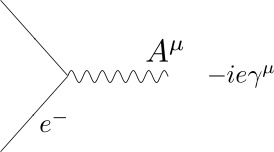
\includegraphics{feynmanruleqed} % in feynmanrules.svf as a Layer
  \caption{Feynman rule for QED}
  \label{fig:feynmanruleqed}
\end{figure}

La repulsión electromagnética esta representada por la figura \ref{fig:qedrepulsion}. En la Figura (a) el primer electrón emite un fotón y se dispersa, mientras que el segundo absorbe el fotón y se dispersa en la dirección opuesta. En la Figura (b) el primer electón absorve el fotón emitido por el segundo electrón. Los dos diagrams se representa por uno único con el fotón en horizontal como se muestra en la Figura (c).

\begin{figure}
  \centering
  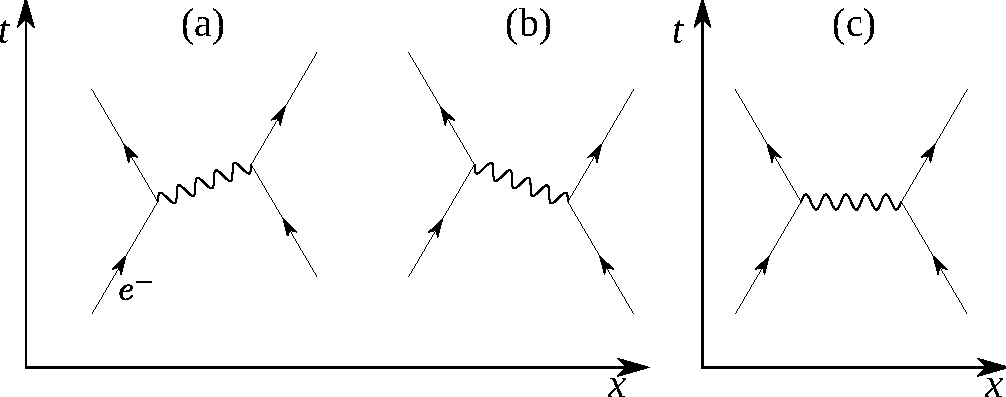
\includegraphics{qedrepulsion}
  \caption{Electromagnetic repulsion. The diagrams (a) and (b) are summarized in the diagram (c)}
  \label{fig:qedrepulsion}
\end{figure}
\end{frame}

\subsection{Paridad}
\begin{align}
  \overline{\psi}\gamma^{\mu}\psi A_{\mu}=&
\xi^{\dagger}\overline{\sigma}^{\mu}\xi A_{\mu}+\eta\sigma^{\mu}\eta^{\dagger} A_{\mu}\nonumber\\
=&(e_L)^{\dagger}\overline{\sigma}^{\mu}e_L A_{\mu}+(e_R)^{\dagger}\sigma^{\mu}e_{R} A_{\mu}\,,
\end{align}
de modo que el fotón se acopla por igual a los campos izquierdos que a los derechos. El Lagrangiano de la QED en términos de espinores de Weyl es:
\begin{align}
  \mathcal{L}_{free}=&i(e_L)^{\dagger}\overline{\sigma}^{\mu}\partial_{\mu}e_L A_{\mu}+i(e_R)^{\dagger}\sigma^{\mu}\partial_{\mu}e_{R}
-m \left[ \left( e_R \right)^\dagger e_L+\left( e_L \right)^{\dagger}e_R \right] -\tfrac{1}{4}F^{\mu\nu}F_{\mu\nu}\nonumber\\
   &+eQ \left[(e_L)^{\dagger}\overline{\sigma}^{\mu}e_L+(e_R)^{\dagger}\sigma^{\mu}e_{R}  \right] A_{\mu}
\end{align}
Se dice entonces que la corriente  electromagnética conserva paridad, es decir es invariante bajo el cambio $L\leftrightarrow R$. 
Una demostración de esta invarianza se muestra en el Apéndice \ref{sec:ferm-quir-de}
%Intentando obtener el operador Hamiltoniano y demás:
%  \begin{align}
%   T^\mu_\nu=&\frac{\partial\mathcal{L}}{\partial\left(\partial_\mu\psi\right)}\partial_\nu\psi+\partial_\nu\bar{\psi}\frac{\partial\mathcal{L}}{\partial\left(\partial_\mu\bar{\psi}\right)}-\mathcal{L}\delta^\mu_\nu\nonumber\\
%   =&i\bar{\psi}\gamma^\mu\partial_\nu\psi-\mathcal{L}\delta^\mu_\nu\,.
% \end{align}
% La expresión para $T^0_i$ es la misma que antes
% \begin{align}
%   T^0_0=i\psi^\dagger\partial_0\psi-i\psi^\dagger\partial_0\psi-i\psi^\dagger\gamma^0\gamma^i\partial_i\psi+m\psi^\dagger\psi-eQ\bar{\psi}\gamma^\mu\psi A_\mu +\tfrac{1}{4}F^{\mu\nu}F_{\mu\nu}.
% \end{align}

En adelante escribiremos el término sólo para el fermión izquierdo $\psi$ (y el correspondiente antifermion derecho $\psi^{\dagger}$

\section{Cromodinámica Cuántica}
\label{sec:inter-fuert}

Como se ilustra en la figura~\ref{fig:crosssection}, en cromodinámica cuántica existe la posibilidad que un electrón y un positrón se aniquilen mutuamente en pura energía llevada por un fotón virtual el cual se debe materializar en un par partícula-antipartícula de acuerdo a la energía disponible. Este es el principio de funcionamiento de los aceleradores electrón-positrón donde se generan dos rayos muy energéticos de electrones y positrones los cuales se hacen colisionar en un punto alrededor de un detector de partículas. El detector esta diseñado para reconstruir los productos de la aniquilación del par electrón positrón. Por ejemplo, si el par electrón-positrón colisiona con una energía superior a $\SI{212}{MeV}$, existe la probabilidad que se cree un par muón ($\mu^-$) antimuón $\mu^{+}$. En teoría cuántica de campos de campos a dicho proceso se le llama sección eficaz y se denota como
\begin{frame}[fragile,allowframebreaks]
\begin{align}
  \sigma(e^+\;e^-\rightarrow \mu^+\;\mu^-)
\end{align}

\begin{figure}
  \centering
  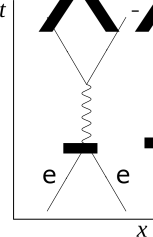
\includegraphics{crosssection}
  \caption{Diagrama de Feynman para la aniquilación electrón-positron y la subsecuente creación de un par partícula-antipartícula de acuerdo a la energía disponible}
  \label{fig:crosssection}
\end{figure}
\end{frame}
Aunque el cálculo de dicho proceso está fuera del alcance de una descripción clásica de los campos, dicha probabilidad debe ser proporcional al cuadrado de la carga eléctrica de la partícula producida, en este caso $Q_{\mu}^2=1$, en unidades de la carga del electrón. El conjunto fermiones elementales que interaccionan sólo de forma electrodébil se conoce como \emph{leptones} y esta especificado en la tabla~\ref{tab:leptons}
\begin{frame}
\begin{figure}
  \centering
  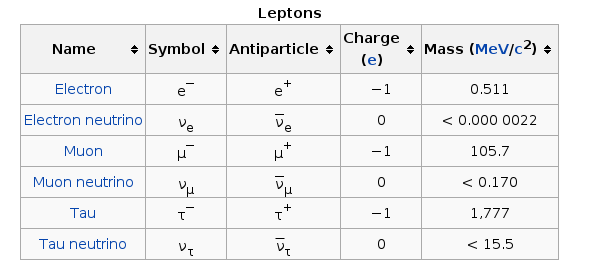
\includegraphics[scale=0.85]{leptons}
  \caption{Leptones de: \url{http://en.wikipedia.org/wiki/List_of_particles}}
  \label{tab:leptons}
\end{figure}
\end{frame}

Con el avance de la tecnología de aceleradores, en la década de los 50 y 60 del siglo pasado se logró establecer la existencia de un zoológico de nuevas partículas, la mayoría de ellas correspondientes a \emph{hadrónes} en el proceso:
\begin{align}
  \sigma(e^+\;e^-\rightarrow \text{hadrónes})\,.
\end{align}
Los protones, neutrones, piones, kaones y demás hadrones, son partículas compuestas de constituyentes elementales llamados quarks. Por ejemplo los protones, neutrones y piones están constituidos de quarks up y down. Los hadrones están dividos en  bariones, $B$, constituidos de tres quarks, y los mesones, $M$, de dos. Para satisfacer el principio de exclusión de Pauli, y justificar el confinamiento de los hadrones, se requiere que cada quark contenga $N_c$ cargas diferentes, llamadas cargas de color, de manera que la carga de color de un hadrón sea cero, de forma similar a como la carga eléctrica de un átomo es cero a pesar de que sus constituyentes poseen carga eléctrica. Muchos resultados experimentales respaldan la existencia de tres cargas de color para cada quark, $N_c=3$. De este modo cada quark $q=u,d,c,s,t,b$, con las propiedades mostradas en la tabla~\ref{tab:quarks}, viene en tres colores
\begin{equation}
  q_\alpha=q_1,q_2,q_3=q_r,q_b,q_g,
\end{equation}
donde los últimos subíndices hacen referencia a los colores red, blue, green. De este modo los Bariones y mesones están descritos por combinaciones singletes de color del tipo $q_r q_b q_g$ y $q_r\bar{q}_r$,
\begin{equation}
\label{eq:199qft}
  B=\frac{1}{\sqrt{6}}\epsilon_{\alpha\beta\gamma}
  \left|q_\alpha q_\beta q_\gamma\right\rangle \qquad M=\frac{1}{\sqrt{3}}\delta^{\alpha\beta}\left|\bar{q}_{\alpha}q_\beta\right\rangle
\end{equation}
Estos estados son singletes de color.

\begin{frame}
\begin{figure}
  \centering
  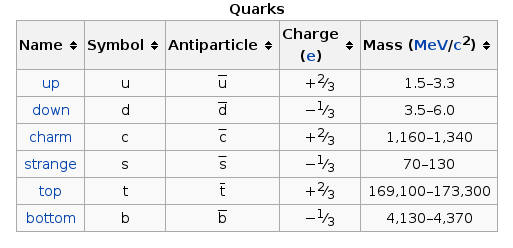
\includegraphics[scale=0.85]{quarks}
  \caption{Quarks de: \url{http://en.wikipedia.org/wiki/List_of_particles}}
  \label{tab:quarks}
\end{figure}
\end{frame}


Una de las determinaciones de $N_c$ proviene del observable
\begin{align}
  R\approx&\frac{\sigma(e^+e^-\to\text{hadrones})}{\sigma(e^+e^-\to\mu^+\mu^-)}
\end{align}

Para $f=u,d,s,c,b,t$, (en orden de masa) tenemos que para una energía donde se pueden producir hadrones compuestos de hasta  quarks $f_{\text{max}}$
\begin{align}
  R\approx&\frac{\sum_{f=u}^{f_{\text{max}}}\sum_{\alpha=1}^{N_c}\sigma(e^+e^-\to f_\alpha\bar{f}_\alpha)}{\sigma(e^+e^-\to\mu^+\mu^-)}\nonumber\\
  R\approx&N_c\frac{\sum_{f=u}^{f_{\text{max}}}\sigma(e^+e^-\to f\bar{f})}{\sigma(e^+e^-\to\mu^+\mu^-)}
\end{align}
De este modo $R$ esta dado por la suma de las cargas eléctricas al cuadrado
\begin{align}
\label{eq:254qft}
R\approx&N_c\frac{\sum_f Q_f^2}{Q_\mu^2}\nonumber\\
=
&N_c\sum_{f=u}^{f_{\text{max}}} Q_f^2\nonumber\\
=&
\begin{cases}
  N_c[(\frac{2}{3})^2+2(\frac{-1}{3})^2]=\frac{2}{3}N_c&f=u,d,s,\;f_{\text{max}}=s\\
  N_c[2(\frac{2}{3})^2+2(\frac{-1}{3})^2]=\frac{10}{9}N_c&f_{\text{max}}=c\\
  N_c[2(\frac{2}{3})^2+3(\frac{-1}{3})^2]=\frac{11}{9}N_c&f_{\text{max}}=b
\end{cases}\nonumber\\
=&
\begin{cases}
  2&N_c=3,\qquad f_{\text{max}}=s\\
  \frac{10}{3}&N_c=3,\qquad f_{\text{max}}=c\\
  \frac{11}{3}&N_c=3,\qquad f_{\text{max}}=b\\
\end{cases}
\end{align}
%\left(\right)
En la figura, tomada de \cite{a}, se muestra el gráfico de $R$ con respecto a $\sqrt{s}$ (la energía de centro de masa de la colisión). Se observan dos escalones, uno que va hasta una energía $\sqrt{s}\approx4\,$GeV que corresponden a $f=u,d,s$, con un $R\approx2$,  y otro hasta $\sqrt{s}\approx40\,$GeV que corresponde a $f=u,d,s,c,b$, con un $R\approx3.7\approx11/3$. Los dos valores de $R$ son compatibles con los esperados de la ec.~\eqref{eq:254qft}. Como referencia también se señalan los valores para $N_c=4$ (en rojo). 
\begin{frame}
\begin{figure}
  \centering
  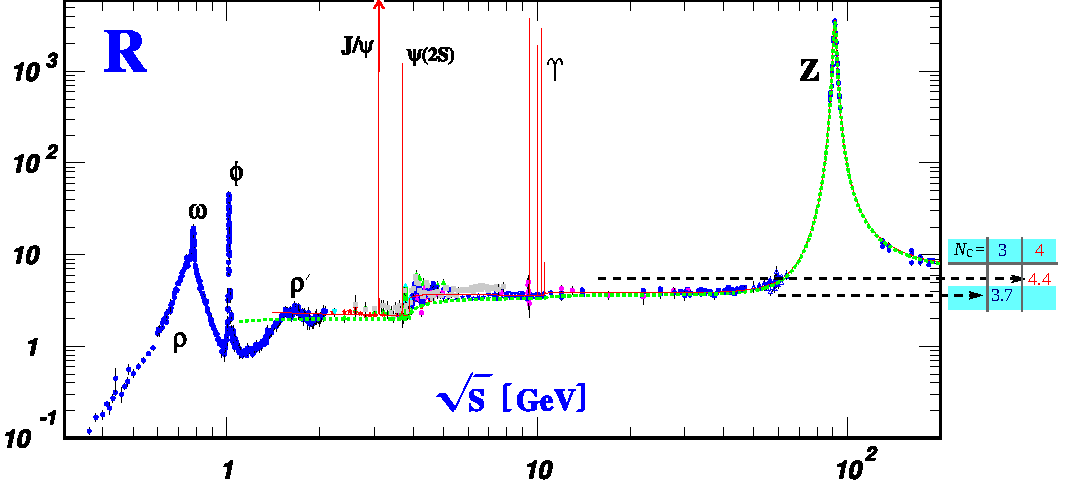
\includegraphics[scale=0.65]{r}
  \caption{Datos para $R$}
  \label{fig:r}
\end{figure}
\end{frame}
\begin{frame}
Si queremos que el color sea una carga conservada como la carga eléctrica, ésta debe ser la consecuencia de una simetría gauge local. Para tener tres cargas diferentes la posibilidad más simple es imponer la simetría $SU(3)_c$, tal que tengamos un vector compuesto de 3 espinores de Dirac en el espacio de color:

  
\begin{equation}
  \Psi=
  \begin{pmatrix}
    \psi_r\\
    \psi_b\\
    \psi_g
  \end{pmatrix}
  =
  \begin{pmatrix}
    q_r\\
    q_b\\
    q_g
  \end{pmatrix}\qquad q=u,d,c,s,t,b\,.
\end{equation}
\end{frame}
El Lagrangiano de Dirac con invarianza gauge global $SU(3)$, para un quark, se puede escribir como
\begin{equation}
  \label{eq:128qft}
  \mathcal{L}_{\text{global}}=i\bar{\Psi}\gamma^\mu\partial_\mu\Psi-m\bar{\Psi}\Psi,
\end{equation}
El análisis es completamente simiar si se usa el Lagrangiano sólo para los fermiones de Weyl izquierdos
\begin{align}
    \mathcal{L}_{\text{global}}=i\bar{\Psi}\overline{\sigma}^\mu\partial_\mu\Psi
\end{align}

\begin{frame}
  
La transformación gauge local bajo $SU(3)$ es
\begin{equation}
  \Psi\to \Psi'=\exp\left(i\theta_a(x)\frac{\lambda^a}{2}\right)\Psi.
\end{equation}
donde $a=1,\ldots,8$, $\lambda_a/2$ son los ocho generadores de $SU(3)$ y $\theta_a(x)$ son los parámetros de la transformación global. Los generadores de $SU(3)$
\begin{align}
  \Lambda^a\equiv\frac{\lambda^a}{2}\,,
\end{align}
satisfacen el álgebra
\begin{equation}
  \left[\frac{\lambda^a}{2},\frac{\lambda^b}{2}\right]=if^{abc}\frac{\lambda^c}{2}\,,
\end{equation}
donde $f^{abc}$ son las constantes de estructura fina de $SU(3)$.
\end{frame}

Las ocho matrices $3\times3$ $\lambda^a$ se pueden construir a partir de las tres matrices de Pauli, pero su forma explícita no es necesaria en la siguiente discusión.

En un análisis similar al de la sección \ref{sec:diracs-lagrangian} tenemos que la Acción invariante gauge local bajo $SU(3)_c$, se obtiene de reemplazar la derivada normal por la derivada covariante. Para compensar los 8 cambios asociados a los 8 parámetros $\theta_a(x)$, la derivada covariante debe definirse en términos de 8 campos vectoriales $G^\nu_a$
\begin{frame}%[fragile,allowframebreaks]
\begin{equation}
  \label{eq:127qft}
  \mathcal{L}_{\text{local}}=i\bar{\Psi}\gamma^\mu\mathcal{D}_\mu\Psi-m\bar{\Psi}\Psi
  -\mathcal{L}\left( G^{\nu}_{a},\partial_{\mu}G^{\nu}_{a} \right)\,.%\frac{1}{2}\operatorname{Tr}\left({G}^{\mu\nu}{G}_{\mu\nu}\right),
\end{equation}
donde
\begin{align}
  \label{eq:qcdtr}
  \Psi\to \Psi'&=U(x)\Psi\nonumber\\
  \mathcal{D}_\mu\Psi\to \left(\mathcal{D}_\mu\Psi\right)'&
  =U(x)\mathcal{D}_\mu\Psi,
\end{align}
con la matriz $3\times 3$
\begin{align}
  U(x)=\exp\left[i\theta_a(x)\frac{\lambda^a}{2}\right]\,,
\end{align}
y
\begin{equation}
  \mathcal{D}_\mu=\partial_\mu-i g_s\frac{\lambda_a}{2}G_\mu^a\equiv\partial_\mu-i g_s {G}_\mu
\end{equation}
donde hemos definido la matriz $3\times 3$  $G_\mu$, como
\begin{equation}
  \left({G}_\mu\right)_{\alpha\beta}=\left(\frac{\lambda_a}{2}\right)_{\alpha\beta}G_\mu^a
\end{equation}
\end{frame}
Este Lagrangiano da lugar a la interacción fuerte y es llamado el Lagrangiano de la Cromodinámica Cuántica, o el Lagrangiano de la QCD de sus siglas en Inglés.

De \eqref{eq:qcdtr}, tenemos
\begin{align}
   \mathcal{D}_\mu\Psi\to \left(\mathcal{D}_\mu\Psi\right)'=&\mathcal{D}'_\mu\Psi'
  =U(x)\mathcal{D}_\mu\Psi\nonumber\\
\mathcal{D}'_\mu U\Psi
  =U(x)\mathcal{D}_\mu\Psi\,.
\end{align}
Por consiguiente
\begin{equation}
  {\mathcal{D}'}^\mu U=U\mathcal{D}^\mu
\end{equation}
\begin{equation}
  \mathcal{D}^\mu\to\left(
    \mathcal{D}^\mu
  \right)'=U\mathcal{D}^\mu U^{-1}
\end{equation}
Desarrollando a ambos lados
\begin{align}
  \label{eq:251qft}
   {\mathcal{D}}^\mu\psi\to{\left({\mathcal{D}}^\mu\psi\right)}'=
  {\mathcal{D}^\mu}'\psi'=&{\mathcal{D}^\mu}'\psi'\nonumber\\
  (\partial^\mu-i g_s {G'}^\mu) U\psi=&U\mathcal{D}^\mu U^{-1}U\psi\nonumber\\
  (\partial^\mu-i g_s {G'}^\mu) U\psi=&U(\partial^\mu-i g_s {G}^\mu)\psi\nonumber\\
  U\partial^\mu\psi+(\partial^\mu U)\psi-i g_s {G'}^\mu U \psi=&U\partial^\mu\phi-i g_s U {G}^\mu \psi\nonumber\\
  (\partial^\mu U)\psi-i g_s {G'}^\mu U \psi=&-i g_s U {G}^\mu \psi\nonumber\\
  -i g_s {G'}^\mu U \psi=&-(\partial^\mu U)\psi-i g_s U {G}^\mu \psi\,,
\end{align}
de modo que
\begin{align}
     {G'}^\mu U =&\frac{1}{i g_s}(\partial^\mu U)+ U{G}^\mu \nonumber\\
   {G'}^\mu  =&-\frac{i}{g_s}(\partial^\mu U)U^{-1}+ U{G}^\mu U^{-1}\,.
\end{align}
\begin{frame}[fragile,allowframebreaks]
Como $U$ es unitaria, la transformación de los campos gauge puede escribirse como
\begin{equation}
    {G}^\mu\to\left({G}^\mu\right)'=U{G}^\mu U^{\dagger}-\frac{i}{g_s}\left(\partial^\mu U\right)U^\dagger.
\end{equation}

Entonces
\begin{align}
\label{eq:Gmuinv}
  \Lambda^a{G'}^\mu_a\approx&(1+i\theta_b\Lambda^b)\Lambda^cG^\mu_c(1-i\theta_d\Lambda^d)-\frac{i}{g_s}[i(\partial^\mu\theta_e)\Lambda^e(1-i\theta_f\Lambda^f)]\nonumber\\
  =&(\Lambda^c+i\theta_b\Lambda^b\Lambda^c)(1-i\theta_d\Lambda^d)G^\mu_c-\frac{i}{g_s}[i(\partial^\mu\theta_e)\Lambda^e(1-i\theta_f\Lambda^f)]\nonumber\\
  \approx&[\Lambda^c-i\theta_d\Lambda^c\Lambda^d+i\theta_b\Lambda^b\Lambda^c]G^\mu_c+\frac{1}{g_s}\Lambda^e\partial^\mu\theta_e\nonumber\\
  =&[\Lambda^c-i\theta_b(\Lambda^c\Lambda^b-\Lambda^b\Lambda^c)]G^\mu_c+\frac{1}{g_s}\Lambda^e\partial^\mu\theta_e\nonumber\\
  =&\Lambda^aG^\mu_a-i(i f^{acb}\Lambda^a)G^\mu_c\theta_b+\frac{1}{g_s}\Lambda^a\partial^\mu\theta_a\nonumber\\
  =&\Lambda^a\left(G^\mu_a+\frac{1}{g_s}\partial^\mu\theta_a+f^{acb}G^\mu_c\theta_b\right)
\end{align}

de donde
\begin{align}
  \label{eq:gmutrinf}
  G^\mu_a\to {G'}^\mu_a\approx&G^\mu_a+\frac{1}{g_s}\partial^\mu\theta_a+{f_a}^{bc}G^\mu_b\theta_c
\end{align}
que se reduce al caso Abeliano cuando las constates de estructura son cero. Como era de esperarse cada campo gauge tiene asociado un parámetro de transformación gauge $\theta_a(x)$.
\end{frame}

\begin{frame}[fragile,allowframebreaks]
  \begin{table}
    \centering
    \begin{tabular}{lll}
      QED & QCD & Diferencia\\\hline
$      \overline{\psi}\left(i\gamma^\mu\mathcal{D}_\mu-m\right)\psi +\mathcal{L} \left(A_{\nu},\partial A_{\nu}  \right)$ & $      \overline{\Psi}\left(i\gamma^\mu\mathcal{D}_\mu-m\right)\Psi +\mathcal{L} \left(G_{\nu},\partial G_{\nu}  \right)$ & $1\times 1 \to 3\times 3$\\ 
$\mathcal{D}_{\mu}=\partial_{\mu}-i e A_{\mu}$ & $\mathcal{D}_{\mu}=\partial_{\mu}-i g G_{\mu}$ & $1\times 1 \to 3\times 3$\\ 
$A_{\mu}\to \widehat{Q}A_{\mu}$ & $G_{\mu}=\Lambda_{a}G_{\mu}^{a}$ & $1\times 1 \to 3\times 3$\\ 
&& $1\to 8\,, a=1,\cdots,8$\\
$    {A}^\mu\to {A}^{\prime\mu}=U{A}^\mu U^{*}-\frac{i}{g_s}\left(\partial^\mu U\right)U^*$&
$ {G}^\mu\to {G}^{\prime\mu}=U{G}^\mu U^{\dagger}-\frac{i}{g_s}\left(\partial^\mu U\right)U^\dagger$
&$1\times 1 \to 3\times 3$\\ 
  $A^\mu\to {A'}^\mu_a\approx A^\mu+\frac{1}{e}\partial^\mu\theta$ &
$G^\mu_a\to {G'}^\mu_a\approx G^\mu_a+\frac{1}{g_s}\partial^\mu\theta_a+{f_a}^{bc}G^\mu_b\theta_c$ &\parbox{3.5cm}{radiación $\to$ ra\-dia\-ción\--ma\-teria}  \\
    \end{tabular}
    \caption{Comparación}
  \end{table}
\end{frame}


\subsection{Tensor cromodinámico}



Note entonces que en el lenguage de los teoremas de noether, el campo $G^{\mu}_{a}$ transforma como un campo material y un campo de radiación a la vez, es decir, su transformación depende tanto del parámetro como de la derivada del parámetro. Por consiguiente, es conveniente definir la derivada covariante del campo $G^{\nu}_{a}$. Para ello es conveniente introducir la representación adjunta.


La representación adjunta de $SU(3)$, consiste en las 8 matrices $8\times 8$
\begin{align}
  \left[  \widetilde{\Lambda}^{a}\right]_{bc}=-i {f^{a}}_{bc}\,.
\end{align}



\textbf{Ejemplo:} Definiendo $\Sigma_i$ como las matrices $3\times3$ generadores de $SU(2)$ en la representaci\'on adjunta
\begin{align}
  (\Sigma_i)_{jk}=-i\epsilon_{ijk}
\end{align}
Debemos comprobar que
\begin{align}
  \left[{\Sigma_i},{\Sigma_j}\right]&=i\epsilon_{ijk}{\Sigma_k}\nonumber\\
  \left[{\Sigma_i},{\Sigma_j}\right]_{lm}&=i\epsilon_{ijk}(\Sigma_k)_{lm}
\end{align}

Ya que
\begin{align}
  \label{eq:167}
  (\Sigma_i\Sigma_j)_{lm}&=(\Sigma_i)_{lk}(\Sigma_j)_{km}=-\epsilon_{ilk}\epsilon_{jkm}=\epsilon_{ilk}\epsilon_{jmk}=\delta_{ij}\delta_{lm}-\delta_{im}\delta_{lj}\nonumber\\
  -(\Sigma_j\Sigma_i)_{lm}&=-(\Sigma_j)_{lk}(\Sigma_i)_{km}=\epsilon_{jlk}\epsilon_{ikm}=-\epsilon_{jlk}\epsilon_{imk}=-\delta_{ji}\delta_{lm}+\delta_{jm}\delta_{li}
\end{align}
Entonces
\begin{align}
[\Sigma_i,\Sigma_j]_{lm}=& (\Sigma_i\Sigma_j-\Sigma_j\Sigma_i)_{lm}\nonumber\\
=&\delta_{il}\delta_{jm}-\delta_{im}\delta_{jl}\nonumber\\
=&\epsilon_{ijk}\epsilon_{lmk}\nonumber\\
=&i\epsilon_{ijk}(-i\epsilon_{klm})\nonumber\\
=&i\epsilon_{ijk}(\Sigma_k)_{lm}
\end{align}


\textbf{Ejercicio:} Demostar que la representación adjunta satisface el álgebra de $SU(3)$


La derivada covariante en la representación adjunta es
\begin{align}
  \mathcal{D}_{\mu}=&\mathbf{1}\partial_{\mu}-i g_s G_{\mu}  \nonumber\\
=&\mathbf{1}\partial_{\mu}-i g_s \widetilde{\Lambda}_a G_{\mu}^{a} \,,
\end{align}
Donde $G_{\mu}$ está ahora en la representación adjunto. En componentes
\begin{align}
 \left[\mathcal{D}_{\mu} \right]^b_c=&\delta^b_c\partial_{\mu}-i g_{s}\left[ \widetilde{\Lambda}_{a} G^a_{\mu} \right]^b_c \nonumber\\
                  =&\delta^b_c\partial_{\mu}- g_{s} {f_{a}}^{bc}  G^a_{\mu} \,.
\end{align}

Cuando esta derivada se aplica al campo de gluones,
\begin{align}
  \mathcal{D}_{\mu}  G_{\nu}=& \left(\mathbf{1}\partial_{\mu}-i g_s  G_{\mu} \right)G_{\nu}
\end{align}

o en componentes
\begin{align}
  \left[ \mathcal{D}_{\mu} \right]^{a}_{b} G_{\nu}^{b}=& \left(\delta^a_b\partial_{\mu}-i g_s \left[ G_{\mu} \right]^{a}_{b} \right)G_{\nu}^{b} \nonumber\\
    =& \left(\delta^a_b\partial_{\mu}-i g_s \left[  \widetilde{\Lambda}_c \right]^a_b G^c_{\mu} \right)G_{\nu}^{a}\,.
\end{align}
Para demostrar que en efecto es una derivada covariante, debemos mostrar que transforma como el campo $G_{\nu}$ 
\begin{align}
 \mathcal{D}_{\mu} G_{\nu}\to   \left(   \mathcal{D}_{\mu} G_{\nu} \right)' =&
\left[\partial_{\mu}-i g_s\left(U G_\mu U^{\dagger}-\frac{i}{g_s}\left(\partial_\mu U\right)U^\dagger  \right)   \right] \left(U G_\nu U^{\dagger}-\frac{i}{g_s}\left(\partial_\nu U\right)U^\dagger  \right) \nonumber\\
=&
\left[\partial_{\mu}-i g_sU G_\mu U^{\dagger}-\left(\partial_\mu U\right)U^\dagger   \right] \left(U G_\nu U^{\dagger}-\frac{i}{g_s}\left(\partial_\nu U\right)U^\dagger  \right) \nonumber\\
=&
\partial_{\mu} \left(U G_\nu U^{\dagger}-\frac{i}{g_s}\left(\partial_\nu U\right)U^\dagger  \right)
-i g_sU G_\mu U^{\dagger}\left(U G_\nu U^{\dagger}-\frac{i}{g_s}\left(\partial_\nu U\right)U^\dagger  \right)
\nonumber\\
&-\left(\partial_\mu U\right)U^\dagger\left(U G_\nu U^{\dagger}-\frac{i}{g_s}\left(\partial_\nu U\right)U^\dagger  \right) \nonumber\\
  =& \cancel{\left(\partial_{\mu} U \right) G_\nu U^{\dagger}} + U
  \left( \partial_{\mu}G_\nu \right) U^{\dagger} + U
  G_{\nu} \partial_{\mu} U^{\dagger} -\frac{i}{g_s}\partial_{\mu}
  \left[ \left( \partial_{\nu}U \right)U^{\dagger} \right]
  \nonumber\\
  &-i g_s U G_{\mu}G_{\nu}U^{\dagger}- UG_{\mu} U^{\dagger} \left( \partial_{\nu} U\right)U^{\dagger} \nonumber\\
  &-\cancel{\left( \partial_{\mu}U \right)G_{\nu} U^{\dagger}}
  +\frac{i}{g_s} \left( \partial_{\mu}U \right) U^{\dagger} \left( \partial_{\nu}U \right) U^{\dagger} \nonumber\\
  =& U \left( \partial_{\mu}G_\nu \right) U^{\dagger} + U
  G_{\nu} \partial_{\mu} U^{\dagger}
  -\cancel{\frac{i}{g_s}\partial_{\mu} \left[ U
      U^{\dagger}\left( \partial_{\nu}U \right)U^{\dagger} \right]}
  \nonumber\\
  &-i g_s U G_{\mu}G_{\nu}U^{\dagger}- UG_{\mu}
  U^{\dagger}\cancel{ \partial_{\nu}\left( UU^{\dagger} \right)}+
  UG_{\mu} U^{\dagger} U\partial_{\nu}U^{\dagger}
  \nonumber\\
  &+\cancel{\frac{i}{g_s} \partial_{\mu} \left[ U U^{\dagger}
      \left( \partial_{\nu}U \right) U^{\dagger}\right]}-
  \frac{i}{g_s} U \partial_{\mu} \left[ U^{\dagger}
    \left( \partial_{\nu}U \right) U^{\dagger}\right]
\end{align}
Ya que
\begin{align}
 \partial_{\mu} \left[ U^{\dagger}
    \left( \partial_{\nu}U \right) U^{\dagger}\right]=&
 \partial_{\mu} \left[ U^{\dagger} U \partial_{\nu} U^{\dagger}\right] \nonumber\\
=& \partial_{\mu}  \partial_{\nu} U^{\dagger} \nonumber\\
\end{align}
entonces
\begin{align}
    \nonumber\\
\mathcal{D}_{\mu} G_{\nu}\to   \left(   \mathcal{D}_{\mu} G_{\nu} \right)' =& U \left[ \left( \partial_{\mu}-ig_s G_{\mu} \right)G_\nu   \right]U^{\dagger}
    + U \left[ G_{\nu} \partial_{\mu}+G_{\mu}\partial_{\nu}-\frac{i}{g_s} \partial_{\mu}\partial_{\nu} \right] U^{\dagger} \nonumber\\
 =& U \left( \mathcal{D}_{\mu}G_\nu   \right)U^{\dagger}
    + U \left[ G_{\nu} \partial_{\mu}+G_{\mu}\partial_{\nu}-\frac{i}{g_s} \partial_{\mu}\partial_{\nu} \right] U^{\dagger} \,.%\nonumber\\
 %  =& U \left( \mathcal{D}_{\mu}G_\nu   \right)U^{\dagger}
 %    + U  G_{\nu} \partial_{\mu}U^{\dagger}-\frac{i}{g_s} U\left(\partial_{\mu}+ig_s G_{\mu} \right)\partial_{\nu}  U^{\dagger} \nonumber\\
 % =& U \left( \mathcal{D}_{\mu}G_\nu   \right)U^{\dagger}
 %  \right]  + U  G_{\nu} \partial_{\mu} U^{\dagger}-\frac{i}{g_s}U \mathcal{D}_{\mu}^{\dagger}\partial_{\nu} U^{\dagger}  \nonumber\\
\end{align} 
De modo que la derivada covariante del campo transforma como el campo. %check mejor


Para el campo electromagnético invariante bajo $\operatorname{U}(1)_Q$, podemos considerar el campo fundamental al tensor de campo electromagnético, que bajo el Grupo de Lorentz transforma como
\begin{align}
  F_{\mu\nu} \to F'_{\mu\nu}=&\partial'_{\mu} A'_{\nu} -\partial'_{\nu} A'_{\mu} \nonumber\\
=&g_{\nu\alpha}\partial'_{\mu} A^{\alpha} -\partial'_{\nu} {A'}_{\mu} \nonumber\\
=&g_{\nu\alpha} { \Lambda_{\mu}}^{\beta}\partial_{\beta} {\Lambda^{\alpha}}_{\gamma} {A}^{\gamma} -\partial'_{\nu} {A'}_{\mu} \nonumber\\
=&g_{\nu\alpha} { \Lambda_{\mu}}^{\beta}\partial_{\beta} {\Lambda^{\alpha}}_{\gamma} g^{\gamma\delta} A_{\delta} -\partial'_{\nu} A'_{\mu} \nonumber\\
  =& { \Lambda_{\mu}}^{\beta}\partial_{\beta}   A_{\delta}{\Lambda_{\nu}}^{\delta} -\partial'_{\nu} A'_{\mu} \nonumber\\
  =& { \Lambda_{\mu}}^{\beta}\partial_{\beta}   A_{\delta}{\left( \Lambda^{-1} \right)^{\delta}}_{\nu} -\partial'_{\nu} A'_{\mu} \,.
\end{align}
Aplicando el resultado al segundo término
\begin{align}
  F_{\mu\nu} \to F'_{\mu\nu} =& { \Lambda_{\mu}}^{\beta}\partial_{\beta}   A_{\delta}{\left( \Lambda^{-1} \right)^{\delta}}_{\nu} 
     - { \Lambda_{\nu}}^{\delta}\partial_{\delta} A_{\beta}{\left( \Lambda^{-1} \right)^{\beta}}_{\mu}  \nonumber\\
  =& { \Lambda_{\mu}}^{\beta} \left( \partial_{\beta}   A_{\delta}-      \partial_{\delta} A_{\beta} \right)
{\left( \Lambda^{-1} \right)^{\delta}}_{\nu} \,.
\end{align}
Finalmente
\begin{align}
  F_{\mu\nu}(x) \to F'_{\mu\nu}(x)  =& { \Lambda_{\mu}}^{\alpha}F_{\alpha\beta}\left( \Lambda^{-1}x \right)\,
                   {\left( \Lambda^{-1} \right)^{\beta}}_{\nu} \,.
\end{align}

De esta forma
\begin{align}
  F_{\mu\nu}F^{\mu\nu}\to   g^{\mu\gamma}g^{\nu\delta} F'_{\mu\nu} F'_{\gamma\delta}=&
  g^{\mu\gamma}g^{\nu\delta} { \Lambda_{\mu}}^{\alpha}  {\left( \Lambda^{-1} \right)^{\beta}}_{\nu}
{ \Lambda_{\gamma}}^{\sigma}  {\left( \Lambda^{-1} \right)^{\rho}}_{\delta}
F_{\alpha\beta}F_{\sigma\rho} \nonumber\\
  =&
   { \Lambda_{\mu}}^{\alpha}  {\left( \Lambda^{-1} \right)^{\beta}}_{\nu}
{ \Lambda^{\mu}}_{\xi}g^{\xi\sigma}  {\left( \Lambda^{-1} \right)_{\eta}}^{\nu}g^{\eta\rho}
F_{\alpha\beta}F_{\sigma\rho}  \nonumber\\
  =& {\left( \Lambda^{-1} \right)^{\alpha}}_{\mu} { \Lambda^{\mu}}_{\xi}
    {\left( \Lambda^{-1} \right)^{\beta}}_{\nu}
 {\Lambda^{\nu}}_{\eta} g^{\xi\sigma}  g^{\eta\rho}
F_{\alpha\beta}F_{\sigma\rho} \nonumber\\
  =& \delta^{\alpha}_{\xi}\delta^{\beta}_{\eta}g^{\xi\sigma}  g^{\eta\rho}
F_{\alpha\beta}F_{\sigma\rho} \nonumber\\
  =& g^{\alpha\sigma}  g^{\beta\rho}
F_{\alpha\beta}F_{\sigma\rho} \nonumber\\
  =& F_{\alpha\beta}F^{\alpha\beta}\,.
\end{align}

Consideremos primero la representación adjunta del álgebra de SU(N):


En SU(N), in conjunto de $N^2-1$ tensores, se puede combinar en una matrix $G^{\mu\nu}$:
\begin{align}
\label{eq:Gmunu}
G^{\mu\nu}=\widetilde{\Lambda}^aG^{\mu\nu}_a
\end{align}

Entonces
\begin{align}
  G_{\mu\nu}\equiv & \mathcal{D}_{\mu} G_{\nu}-\mathcal{D}_{\nu} G_{\mu} \nonumber\\
=&\left( \mathbf{1}\partial_{\mu}-i g_s G_{\mu} \right)G_{\nu}-
\left( \mathbf{1}\partial_{\nu}-i g_s G_{\nu} \right)G_{\mu}\nonumber\\
=& \partial_{\mu}G_{\nu}-\partial_{\nu}G_{\mu}
-ig_s \left(  G_{\mu}G_{\nu}-G_{\nu}G_{\mu}  \right) \nonumber\\
=& \partial_{\mu}G_{\nu}-\partial_{\nu}G_{\mu}
-ig_s \left[  G_{\mu},G_{\nu}  \right] .
\end{align}
De manera que
\begin{align}
  \widetilde{\Lambda}_a G_{\mu\nu}^a=& \widetilde{\Lambda}_a
\left( \partial_{\mu}G_{\nu}^{a}-\partial_{\nu}G_{\mu}^{a}  \right)
-i g_s \left[ \widetilde{\Lambda}_b,\widetilde{\Lambda}_c \right]G_{\mu}^{b}G_{\nu}^{c} \nonumber\\
=&\widetilde{\Lambda}_a
\left( \partial_{\mu}G_{\nu}^{a}-\partial_{\nu}G_{\mu}^{a}  \right)
-i g_s \left(i {f^{a}}_{bc} \widetilde{\Lambda}_a \right)G_{\mu}^{b}G_{\nu}^{c} \,.
\end{align}
Entonces
\begin{align}
  G_{\mu\nu}^a=\partial_{\mu}G_{\nu}^{a}-\partial_{\nu}G_{\mu}^{a}+
g_s{f^{a}}_{bc}G_{\mu}^{b}G_{\nu}^{c} \,.
\end{align}
El tensor \eqref{eq:Gmunu} debe transformar en la representación adjunta de $\operatorname{SU}(N)$ como
\begin{align}
\label{eq:pGmunu}
  G^{\mu\nu}\to  {G'}^{\mu\nu}=U  G^{\mu\nu} U^{-1}
\end{align}
La transformación \eqref{eq:pGmunu} es consisitente con
\begin{align}
  G^{\mu}\to {G'}^{\mu}= U G^{\mu} U^{-1}
-\frac{i}{g_s} \left( \partial_{\mu} U \right) U^{-1}
\end{align}


Para poder obtener un invariante bajo transformaciones gauge a partir del producto $G^{\mu\nu}G_{\mu\nu}$, debemos utilizar la traza 
\begin{align}
  \operatorname{Tr}\left(G^{\mu\nu}G_{\mu\nu}\right)\to
  \operatorname{Tr}\left({G\,'}^{\mu\nu}{G\,'}_{\mu\nu}\right)
  =&\operatorname{Tr}\left(U{{G}}^{\mu\nu}U^{-1}U{{G}}_{\mu\nu}U^{-1}\right)\nonumber\\
  =&\operatorname{Tr}\left(U{{G}}^{\mu\nu}{{G}}_{\mu\nu}U^{-1}\right)\nonumber\\
  =&\operatorname{Tr}\left(U^{-1}U{{G}}^{\mu\nu}{{G}}_{\mu\nu}\right)\nonumber\\
  =&\operatorname{Tr}\left({{G}}^{\mu\nu}{{G}}_{\mu\nu}\right)\,.
\end{align}
Teniendo en cuenta la normalización de las matrices de SU(3) (Las relaciones siguientes son independientes de la representación y por lo tanto omitiremos la tilda para la representación adjunta)
\begin{align}
   \operatorname{Tr}\left(\Lambda^a\Lambda^b\right)=&\frac{1}{2}\delta^{ab}\,,
\end{align}
tenemos (suma sobre indices repetidos de $SU(3)$)
\begin{align}
  \operatorname{Tr}\left(G^{\mu\nu}G_{\mu\nu}\right)\to
  \operatorname{Tr}\left({G\,'}^{\mu\nu}{G\,'}_{\mu\nu}\right)
  =&\operatorname{Tr}\left(\Lambda^a{G}^{\mu\nu}_a \Lambda^b{G}_{\mu\nu}^b\right)\nonumber\\
  =&\operatorname{Tr}\left(\Lambda^a \Lambda^b\right){G}^{\mu\nu}_a {G}_{\mu\nu}^b\nonumber\\
  =&\frac{1}{2}\delta^{a b}{G}^{\mu\nu}_a {G}_{\mu\nu}^b\nonumber\\
  =&\frac{1}{2}{G}^{\mu\nu}_a {G}_{\mu\nu}^a\,.
\end{align}
Haciendo explícitamente la traza tenemos (suma sobre índices $a,b,c,\cdots$ repetidos aunque no estén contraidos)
\begin{align}
  {G}^{\mu\nu}_a {G}_{\mu\nu}^a=&
\left( \widetilde{G}^{\mu\nu}_a+g_s f^{abc}G^\mu_b G^\nu_c, \right)
\left( \widetilde{G}_{\mu\nu}^a+g_s f_{ade}G_\mu^d G_\nu^e, \right) \nonumber\\
=&\widetilde{G}^{\mu\nu}_a\widetilde{G}_{\mu\nu}^a+g_s f_{ade}\widetilde{G}^{\mu\nu}_aG_\mu^d G_\nu^e
+g_s f^{abc}\widetilde{G}_{\mu\nu}^a G^\mu_b G^\nu_c +g_s^2 f^{abc}f_{ade}G^\mu_b G^\nu_c G_\mu^d G_\nu^e 
\nonumber\\
=&\widetilde{G}^{\mu\nu}_a\widetilde{G}_{\mu\nu}^a+g_s f^{abc}\widetilde{G}^{\mu\nu}_aG_\mu^b G_\nu^c
+g_s f^{abc}\widetilde{G}_{\mu\nu}^a G^\mu_b G^\nu_c +g_s^2 f^{abc}f_{ade}G^\mu_b G^\nu_c G_\mu^d G_\nu^e 
\nonumber\\
=&\widetilde{G}^{\mu\nu}_a\widetilde{G}_{\mu\nu}^a+g_s f^{abc}\widetilde{G}^{\mu\nu}_aG_\mu^b G_\nu^c
+g_s f^{abc}\widetilde{G}^{\mu\nu}_aG_\mu^b G_\nu^c +g_s^2 f^{abc}f_{ade}G^\mu_b G^\nu_c G_\mu^d G_\nu^e 
\nonumber\\
=&\widetilde{G}^{\mu\nu}_a\widetilde{G}_{\mu\nu}^a+2g_s f^{abc}\widetilde{G}^{\mu\nu}_aG_\mu^b G_\nu^c
+g_s^2 f^{abc}f_{ade}G^\mu_b G^\nu_c G_\mu^d G_\nu^e 
\end{align}

\subsection{Lagrangiano QCD}

\begin{frame}[fragile,allowframebreaks]
Expandiendo el Lagrangiano en ec.~(\ref{eq:127qft}), tenemos
\begin{align}
  \mathcal{L}=&i\bar{\Psi}\gamma^\mu\left(\partial_\mu-i g_s\frac{\lambda_a}{2}G_\mu^a\right)\Psi
  -m\bar{\Psi}\Psi- \frac{1}{2}\operatorname{Tr}\left(G^{\mu\nu} G_{\mu\nu}\right)\nonumber\\
  =&i\bar{\Psi}\gamma^\mu\left(\partial_\mu-i g_s\frac{\lambda_a}{2}G_\mu^a\right)\Psi
  -m\bar{\Psi}\Psi- \frac{1}{4}G^{\mu\nu}_a G_{\mu\nu}^a\nonumber\\
=&i\bar{\Psi}\gamma^\mu\partial_\mu\Psi-m\bar{\Psi}\Psi+g_s\bar{\Psi}\gamma^\mu\frac{\lambda_a}{2}G_\mu^a\Psi
  - \frac{1}{4}G^{\mu\nu}_a G_{\mu\nu}^a\nonumber\\
=&i\bar{\Psi}\gamma^\mu\partial_\mu\Psi-m\bar{\Psi}\Psi+g_s\bar{\Psi}\gamma^\mu\frac{\lambda_a}{2}\Psi G_\mu^a
  - \frac{1}{4}\widetilde{G}^{\mu\nu}_a \widetilde{G}_{\mu\nu}^a\nonumber\\
  &- \frac{1}{4}\left(%g_s\widetilde{G}^{\mu\nu}_af_{a d e}G^d_\mu G^e_\nu+
    2g_sf^{a b c}G_b^\mu G_c^\nu\widetilde{G}_{\mu\nu}^a
    +g_s^2f^{a b c}f_{a d e}G_b^\mu G_c^\nu G^d_\mu G^e_\nu\right)\nonumber\\
=&\mathcal{L}_{\text{free}}+\mathcal{L}_{\text{gauge}}+\mathcal{L}_{\text{SI}}\,,
\end{align}
donde

\begin{align}
\label{eq:qcdgauge}
\mathcal{L}_{\text{free}}=&i\bar{\Psi}\gamma^\mu\partial_\mu\Psi-m\bar{\Psi}\Psi\nonumber\\
  \mathcal{L}_{\text{gauge}}=&g_s\bar{\Psi}\gamma^\mu\frac{\lambda_a}{2}\Psi G_\mu^a
  - \frac{1}{4}\widetilde{G}^{\mu\nu}_a \widetilde{G}_{\mu\nu}^a\nonumber\\
  \mathcal{L}_{\text{SI}}=&{\color{red}- \frac{1}{4}\left(%g_s\widetilde{G}^{\mu\nu}_af_{a d e}G^d_\mu G^e_\nu+
    2 g_sf^{a b c}G_b^\mu G_c^\nu\widetilde{G}_{\mu\nu}^a
    +g_s^2f^{a b c}f_{a d e}G_b^\mu G_c^\nu G^d_\mu G^e_\nu\right)\,.}
\end{align}

Hemos divido el Lagrangiano en tres partes
\begin{itemize}
\item El Lagrangiano libre de Dirac
\item Una parte gauge que puede escribirse como un Lagrangiano electromagnético:
\begin{align}
  \mathcal{L}_{\text{gauge}}=&-\frac{1}{4}\left(\partial^\mu G^\nu_a-\partial^\nu G^\mu_a\right)\left(\partial_\mu G_\nu^a-\partial_\nu G_\mu^a\right)-J^\nu_aG_\nu^a,
\end{align}
dende
\begin{align}
  J^\mu_a=-g_s\bar{\Psi}\gamma^\mu\frac{\lambda_a}{2}\Psi\,,
\end{align}
es la nueva corriente conservada de interacción fuerte que surge como consecuencia de la invarianza gauge local $SU(3)$; y 
\item Una parte de auto-interacciones gauge:
  \begin{align}
    \mathcal{L}_{\text{SI}}  &=- \frac{g_s}{2}f^{a b c}\widetilde{G}_{\mu\nu}^aG_b^\mu G_c^\nu
    -\frac{g_s^2}{4}f^{a b c}f_{a d e}G_b^\mu G_c^\nu G^d_\mu G^e_\nu\nonumber\\
  &=-\frac{g_s}{2}f^{abc}\left(\partial^\mu G^\nu_a-\partial^\nu G^\mu_a\right)G^b_\mu G^c_\nu-\frac{g_s^2}{4}f^{abc}f_{ade}G^\mu_bG^\nu_cG^d_\mu G^e_\nu.
  \end{align}
que se desaparecen en el caso Abeliano.
\end{itemize}

El Lagrangiano de interacción es:
\begin{align}
  \mathcal{L}_{\text{int}}=g_s\bar{\Psi}\gamma^\mu\frac{\lambda_a}{2}\Psi G_\mu^a-\frac{g_s}{2}f^{abc}\left(\partial^\mu G^\nu_a-\partial^\nu G^\mu_a\right)G^b_\mu G^c_\nu-\frac{g_s^2}{4}f^{abc}f_{ade}G^\mu_bG^\nu_cG^d_\mu G^e_\nu.
\end{align}

%ver la discusión en el libro de Feyman sobre QED
\end{frame}

\begin{frame}
From \cite{Feynman:1986er} (pag 136):
\begin{quote}
  The quarks have an additional type of polarization that is not
  related to geometry. The idiot physicists, unable to come up with
  any wonderful Greek words anymore, call this type of polarization by
  the unfortunate name of ``color'', which has nothing to do with
  color in the nornal sense. At a particular time, a quark can be in
  one of three conditions, or ``colors''--R, G, or B (can you guess
  what they stand for?). A quark's ``color'' can be changed when the
  quark emits or absorbs a gluon. The gluons come in eigth diffent
  types, according to the ``colors'' they can couple with. For
  example, if a red quark changes to green, it emits a red-antigreen
  gluon--a gluon that takes the red from quark and gives it green
  (``antigreen'' means the gluon is carrying green in the opposite
  direction). This gluon could be absorved by a green quark, which
  changes to red (see Fig.~\ref{fig:qcd}). There are eigth different
  possible gluons, such as red-antired, red-antiblue, red-antigreen,
  and so on (you'd think there'd be nine, but for technical reasons,
  one is missing)\footnote{Ver ec.~\ref{eq:glu}.}. The theory is not very complicated.  The complete rule of gluons is: gluons couple with things having ``color''--it just requires a little bookkeeping to keep track of where the ``colors go''.  There is, however, an interesesting possibility created by this rule: gluons can couple with other gluons (see Fig.~\ref{fig:qcd3gluon}).
\end{quote}
\end{frame}
%11 12 13
%21 22 23
%31 32 33
%33+11+22=0



El primer término da lugar a interacciones de cambio de color de quarks como la que se ilustra en la Figura \ref{fig:qcd}
\begin{frame}  
    \begin{align}
\label{eq:glu}
      \begin{pmatrix}
        \color{red}{r\bar{r}} & \color{red}{r}\bar{b} &\color{red}{r}\bar{g}\\ 
        \color{blue}{b}\color{red}{\bar{r}} & \color{blue}{b\bar{b}} &\color{blue}{b}\color{green}{\bar{g}}\\ 
        \color{green}{g}\color{red}{\bar{r}} & g\color{blue}{\bar{b}} &\color{green}{g\bar{g}}\\ 
      \end{pmatrix},\qquad\text{with}\quad 
      \color{red}{r\bar{r}}+\color{blue}{b\bar{b}}+\color{green}{g\bar{g}}=0\,.
    \end{align}

\begin{figure}
  \centering
  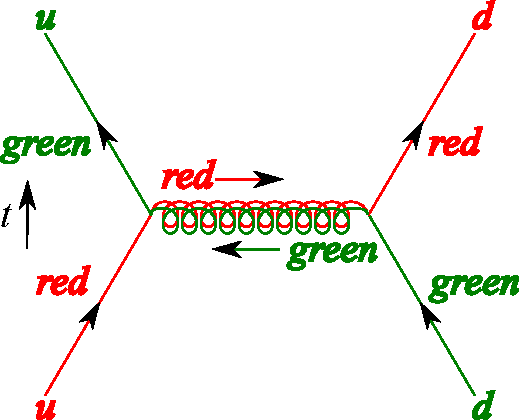
\includegraphics[scale=0.8]{qcd} % In qcd.svg as a layer
  \caption{Quark--gluon interaction}
  \label{fig:qcd}
\end{figure}
\end{frame}
Mientras que el segundo y tercer término dan lugar a autointeracciones de los gluones como se muestra en la Figura \ref{fig:qcd3gluon}
\begin{frame}
\begin{figure}
  \centering
  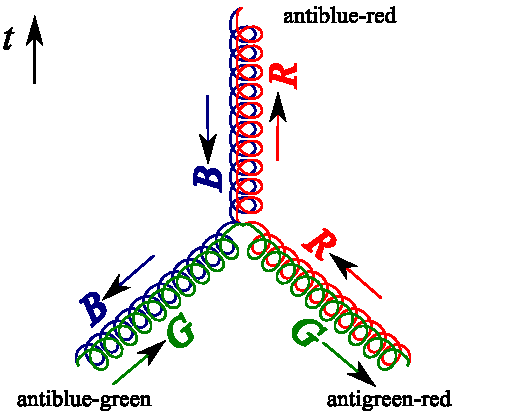
\includegraphics{qcd3gluon}% In qcd.svg as a layer
  \caption{Triple--gluon self--interaction. The anticolors are the colors running back in time.}
  \label{fig:qcd3gluon}
\end{figure}
\end{frame}

Estás interacciones dan lugar a la estructura interna del protón mostrada en la figura~\ref{fig:prt}.

\begin{frame}
  \begin{figure}
    \centering
  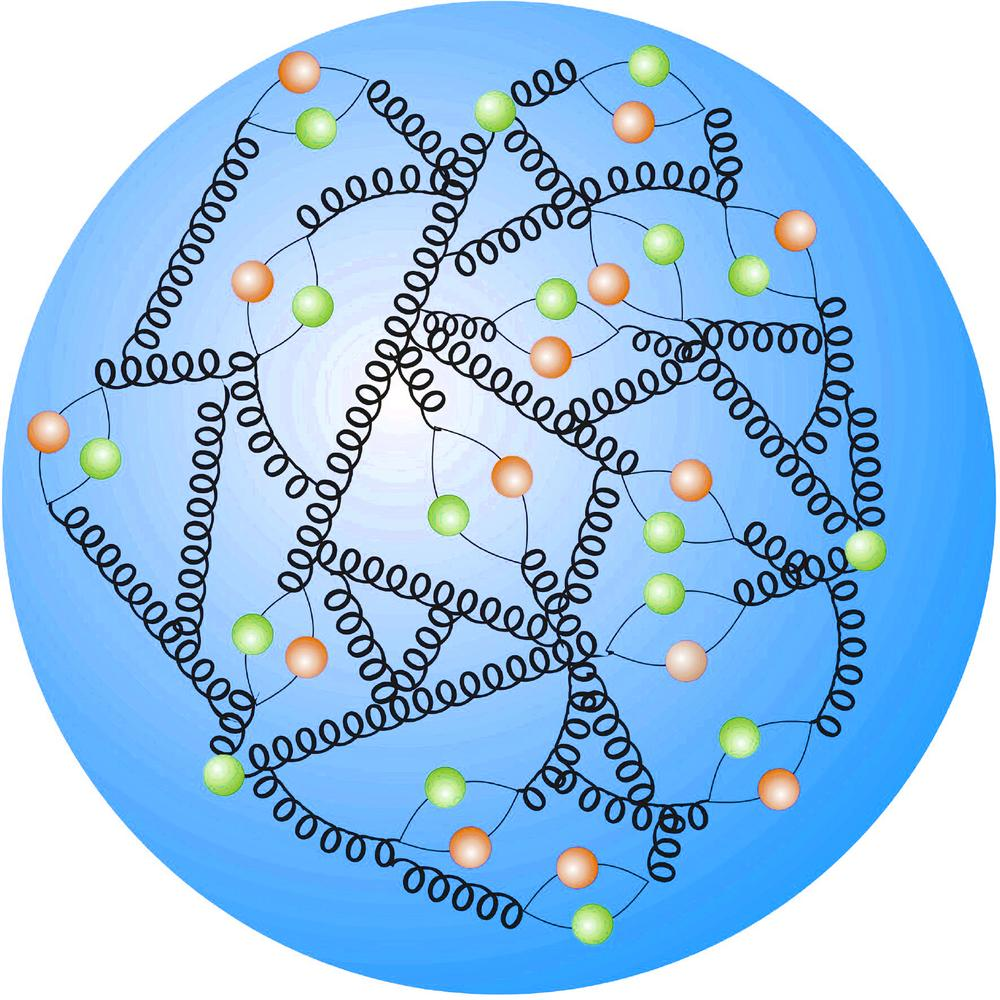
\includegraphics[scale=0.2]{proton}    
    \caption{En la esctructura interna del protón, además de los tres quarks de valencia representados en la figura como las tres partículas verdes aisladas, también están los gluones y los pares quark-antiquark. Estos últimos representados como las partículas naranja. Fuente: \href{http://www.desy.de/news/news_search/index_eng.html?openDirectAnchor=829}{desy.de}}
    \label{fig:prt}
  \end{figure}

\end{frame}

Todas las interacciones están determinadas en términos de una única constante de acoplamiento $g_s$. Las autointeracciones gauge pueden explicar aspectos de la interacción fuerte como la libertada asintótica, que consiste en que las interacciones fuertes se vuelven más débiles a distancias cortas. 

En términos de índices de color la corriente, y las otras partes del Lagrangiano, pueden escribirse como
\begin{equation}
  \label{eq:223qft}
  J^\mu_a=-g_s\bar{q}^\alpha\gamma^\mu q^\beta\left(\frac{\lambda_a}{2}\right)_{\alpha\beta}.
\end{equation}
Note que tanto para la Electrodinámica Cuántica como para la Cromodinámica Cuántica la corriente $\bar{\psi}\Gamma\psi$ es vectorial. Para las interacciones débiles la estructura es más complicada y requiere un conocimiento más profundo de la ecuación de Dirac y sus soluciones.


\subsection{Derivación alternativa}






% \begin{align}
%     \left[ \mathcal{D}_{\mu} \right]_{a}^{b} G^{\nu}_{b}\to 
%    \left\{   \left[ \mathcal{D}_{\mu} \right]_{a}^{b} G^{\nu}_{b}\right\}'=
% \left[ \mathcal{D}_{\mu} \right]_{a}^{b} G^\mu_b+\frac{1}{g_s}\partial^\mu\theta_a
% +f^{abc}\theta_c\left[ \mathcal{D}_{\mu} \right]_{b}^{d} G^\mu_d
% \end{align}
% Esta propiedad puede ser obtenida si usamos 

Algunas identidades útiles en SU(N) son:

\begin{itemize}
\item 
\begin{align}
  \left\{ \Lambda^{a},\Lambda^{b} \right\}=\frac{1}{N}\delta^{ab}+{d^{ab}}_c \Lambda^{c}\,
\end{align}
donde $d^{abc}$ es totalmente simétrico en $a,b,c$

 En el caso de $SU(2)$ $d^{ijk}=0$, 

Para  $SU(2)$
\begin{align}
\left\{T_i,T_j\right\}=\frac{1}{2}\delta_{ij}\mathbf{1}\,.
\end{align}
Para  $SU(3)$
\begin{align}
\left\{\Lambda_a,\Lambda_b\right\}=\frac{1}{3}\delta_{ab}\mathbf{1}+{d^{ab}}_c \Lambda^{c}\,.
\end{align}

\item 
\begin{align}
  f^{abe}f^{cde}=\frac{2}{N}(\delta^{ac}\delta^{bd}-
 \delta^{ad}\delta^{bc})+d^{ace}d^{bde}-d^{ade}d^{bce}
\end{align}
\end{itemize}



Similarmente, definiendo la matriz $3\times 3$, 
\begin{align}
  \label{eq:gmunu}
  {{G}}^{\mu\nu}&=\frac{i}{g_s}[\mathcal{D}^\mu,\mathcal{D}^\nu]\equiv\frac{\lambda_a}{2}G^{\mu\nu}_a,
\end{align}
tenemos
\begin{align}
  \label{eq:164qft}
   {G}^{\mu\nu}\psi =&\frac{i}{g_s}[\partial^\mu-ig_sG^\mu,\partial^\nu-ig_sG^\nu]\psi\nonumber\\
  =&\frac{i}{g_s}\left[\left(\partial^\mu-ig_sG^\mu\right)\left(\partial^\nu-ig_sG^\nu\right)\psi
    -\left(\partial^\nu-ig_sG^\nu\right)\left(\partial^\mu-ig_sG^\mu\right)\psi\right]\nonumber\\
  =&\frac{i}{g_s}\left\{\partial^\mu\partial^\nu\psi-g_s^2G^\mu G^\nu\psi-ig_s[\partial^\mu(G^\nu\psi)+G^\mu\partial^\nu\psi]
    -\partial^\nu\partial^\mu\psi+g_s^2G^\nu G^\mu\psi+ig_s[\partial^\nu(G^\mu\psi)+G^\nu\partial^\mu\psi]\right\}\nonumber\\
  =&\frac{i}{g_s}\{(\partial^\mu\partial^\nu-\partial^\nu\partial^\mu)\psi-g_s^2(G^\mu G^\nu-G^\nu G^\mu)\psi
  -ig_s[(\partial^\mu G^\nu)-(\partial^\nu G^\mu)]\psi\nonumber\\
  &-ig_s[G^\nu\partial^\mu\psi+G^\mu\partial^\nu\psi-G^\mu\partial^\nu\psi+G^\nu\partial^\mu\psi]\}\nonumber\\
=&[\partial^\mu G^\nu-\partial^\nu G^\mu-ig_s(G^\mu G^\nu-G^\nu G^\mu)]\psi\nonumber\\
=&\{\partial^\mu G^\nu-\partial^\nu G^\mu-ig_s[G^\mu,G^\nu]\}\psi
\end{align}

De modo que
\begin{align}
  {G}^{\mu\nu}=&\partial^\mu G^\nu-\partial^\nu G^\mu-ig_s[G^\mu,G^\nu]\,,
\end{align}
que se reduce al caso Abeliano cuando los bosones gauge conmutan. En términos de componentes
\begin{align}
  \Lambda^a{G}^{\mu\nu}_a=&\Lambda^a\partial^\mu G^\nu_a-\Lambda^a\partial^\nu G^\mu_a-ig_s[\Lambda^bG^\mu_b,\Lambda^cG^\nu_c]\nonumber\\
  =&\Lambda^a\partial^\mu G^\nu_a-\Lambda^a\partial^\nu G^\mu_a-ig_s[\Lambda^b,\Lambda^c]G^\mu_bG^\nu_c\nonumber\\
  =&\Lambda^a\partial^\mu G^\nu_a-\Lambda^a\partial^\nu G^\mu_a-ig_s(i\Lambda^af_{a b c})G^\mu_bG^\nu_c\nonumber\\
  =&\Lambda^a\partial^\mu G^\nu_a-\Lambda^a\partial^\nu G^\mu_a+\Lambda^ag_sf_{a b c}G^\mu_bG^\nu_c\,.
\end{align}
Por consiguiente
\begin{equation}
  \label{eq:258qft}
  G^{\mu\nu}_a=\partial^\mu G^\nu_a-\partial^\nu G^\mu_a+g_s f^{abc}G^\mu_b G^\nu_c\equiv\widetilde{G}^{\mu\nu}_a+g_s f^{abc}G^\mu_b G^\nu_c,
\end{equation}
con
\begin{equation}
  \widetilde{G}^{\mu\nu}_a=\partial^\mu G^\nu_a-\partial^\nu G^\mu_a
\end{equation}



A diferencia del caso Abeliano $G^{\mu\nu}$ ya no es invariante bajo transformaciones gauge
\begin{align}
G^{\mu\nu}\to    {G'}^{\mu\nu}
  &=\frac{i}{g_s}\left[{\mathcal{D}'}^\mu,{\mathcal{D}'}^\nu\right]\nonumber\\
&=\frac{i}{g_s}\left[U{\mathcal{D}}^\mu U^{-1},U{\mathcal{D}}^\nu U^{-1}\right]\nonumber\\
&=U{{G}}^{\mu\nu}U^{-1}\,.
\end{align}

Note que con la definición \eqref{eq:gmunu}, la derivada covariante de la matrix $G^{\mu\nu}$, transforma como la matrix $G^{\mu\nu}$
\begin{align}
\mathcal{D}_\mu G^{\mu\nu} \to\left(\mathcal{D}_\mu G^{\mu\nu}\right)'=U\mathcal{D}_\mu G^{\mu\nu} U^{-1}\,.
\end{align}




% La derivada covariante del campo tensorial transforma igual:
% \begin{align}
%  \mathcal{D}_{\mu} G^{\mu\nu}\to  \left( \mathcal{D}_{\mu} G^{\mu\nu}\right)'=U \left( \mathcal{D}_{\mu}G^{\mu\nu} \right) U^{-1}
% \end{align}
% Es interesante notar que
% \begin{align}
%    \mathcal{D}_{\mu} G^{\mu\nu}=& \left(\mathbf{1}\partial_{\mu}-i g_s G_{\mu}  \right) G^{\mu\nu} \nonumber\\
% =& \partial_{\mu}G^{\mu\nu}-i g_s G_{\mu}G^{\mu\nu}\,.
% \end{align}
% De modo que
% \begin{align}
% \mathcal{D}_{\mu} G^{\mu\nu}\to {\left[ \mathcal{D}_{\mu} \right]^{a}}_{b} {\left[ G^{\mu\nu} \right]^{b}}_{c}
% =&\left( \delta^a_b\partial_{\mu}-ig_s {\left[ \widetilde{\Lambda}_e \right]^a}_b G_{\mu}^e \right)  {\left[ \widetilde{\Lambda}^f\right]^{b}}_{c} G^{\mu\nu}_{f}
% \end{align}
% \begin{align}
% =&   \delta^a_b{\left[ \widetilde{\Lambda}^f\right]^{b}}_{c}\partial_{\mu}  G^{\mu\nu}_{f}-ig_s {\left[ \widetilde{\Lambda}_e \right]^a}_b {\left[ \widetilde{\Lambda}^f\right]^{b}}_{c} G_{\mu}^e  G^{\mu\nu}_{f} 
% \end{align}


\section{Soluciones a la ecuaci\'on de Dirac}
\label{sec:soluc-la-ecuac}

\subsection{Lagrangiano de Weyl}
\label{sec:lagrangiano-de-weyl}
\begin{borrar}
En la ec.~\eqref{eq:118}, obtuvimos el Hamiltoniano en ec.~\eqref{eq:103}
\begin{equation}
  \hat{H}= \gamma_0(\boldsymbol{\gamma}\cdot\mathbf{p}+m)=\boldsymbol{\alpha}\cdot\mathbf{p}+\beta m\,.
\end{equation}
Una escogencia particular de las cuatro matrices $\gamma^\mu$, conocida como la representaci\'on de Weyl, o representaci\'on quiral, puede escribirse en t\'erminos de la matrices de Pauli. Escritas en bloques $2\times2$, tenemos
\begin{equation}
  \gamma^0=
  \begin{pmatrix}
    0&\sigma_0\\
    \sigma_0&0
  \end{pmatrix}\qquad
  \gamma_i=\begin{pmatrix}
    0&\sigma_i\\
    -\sigma_i&0
  \end{pmatrix}.
\end{equation}
Con $\sigma^0=1$. Con la matriz de tranformaci\'on
\begin{equation}
  U=\frac{1}{\sqrt{2}}
  \begin{pmatrix}
    1&1\\
    -1&1    
  \end{pmatrix}
\end{equation}
podemos obtener la representaci\'on de Dirac, tal que $U$ diagonaliza $\gamma^0$,
\begin{equation}
  \gamma^0=
  \begin{pmatrix}
    \sigma^0&0\\
    0&-\sigma^0
  \end{pmatrix}\qquad
  \gamma_i=\begin{pmatrix}
    0&\sigma_i\\
    -\sigma_i&0
  \end{pmatrix}.
\end{equation}
\end{borrar}
En adelante trabajaremos en la representaci\'on de Weyl que en forma compacta es
\begin{equation}
  \gamma^\mu=\begin{pmatrix}
    0&\sigma^\mu\\
    \bar{\sigma}^\mu & 0
  \end{pmatrix}
\end{equation}
donde
\begin{align}
  \sigma^\mu&=(\sigma^0,\sigma^1,\sigma^2,\sigma^3)\nonumber\\
  \bar{\sigma}^\mu&=(\sigma^0,-\sigma^1,-\sigma^2,-\sigma^3)\nonumber\\
\end{align}
Hemos escrito las matrices de Dirac en bloques $2\times2$, y es natural escribir similarmente las cuatro componentes del campo de Dirac como un par de campos de dos componentes
\begin{align}
  \psi=  \begin{pmatrix}
    \psi_L\\
    \psi_R    
  \end{pmatrix}=\begin{pmatrix}
    \psi_L\\
    0   
  \end{pmatrix}+\begin{pmatrix}
    0\\
    \psi_R    
  \end{pmatrix}
\end{align}
Donde $\psi_{L,R}$ son espinores de Weyl de dos componentes. En la representaci\'on de Weyl el Lagrangiano se puede escribir como
\begin{align}
\label{eq:200}
  \mathcal{L}=&i\bar{\psi}\gamma^\mu\partial_\mu\psi-m\bar{\psi}\psi\nonumber\\
  =&i\psi^\dagger \gamma^0\gamma^\mu\partial_\mu\psi-m\psi^\dagger \gamma^0 \psi\nonumber\\
  =&i\psi^\dagger  \begin{pmatrix}
    0 & 1\\
    1&0
  \end{pmatrix}
  \begin{pmatrix}
    0 &\sigma^\mu \\
    \bar{\sigma}^\mu&0
  \end{pmatrix}\partial_\mu\psi-m\psi^\dagger
  \begin{pmatrix}
    0 & 1\\
    1&0
  \end{pmatrix}\psi\nonumber\\
=&i\begin{pmatrix}
 \psi_L^\dagger & \psi_R^\dagger
\end{pmatrix}
 \begin{pmatrix}
   \bar{\sigma}^\mu &0\\
   0&\sigma^\mu
 \end{pmatrix} \begin{pmatrix}
   \partial_\mu\psi_L\\
   \partial_\mu\psi_R
 \end{pmatrix}-m
 \begin{pmatrix}
   \psi_L^\dagger&\psi_R^\dagger
 \end{pmatrix}
 \begin{pmatrix}
   0&1\\
   1&0
 \end{pmatrix}
 \begin{pmatrix}
   \psi_L\\ \psi_R
 \end{pmatrix}\nonumber\\
 =& i\psi_L^\dagger \bar{\sigma}^\mu\partial_\mu\psi_L+i\psi_R^\dagger \sigma^\mu\partial_\mu\psi_R
  -m(\psi_L^\dagger \psi_R+\psi_R^\dagger \psi_L)
\end{align}

\subsection{Ecuaciones de Weyl}
\label{sec:ecuaciones-de-weyl}
Las ecuaciones de Euler-Lagrango para el Lagrangiano en ec.\eqref{eq:200}, dan como resultado
\begin{align}
  i\bar{\sigma}^\mu\partial_\mu\psi_L -m\psi_R &=0\nonumber\\
  i{\sigma}^\mu\partial_\mu\psi_R -m\psi_L &=0
\end{align}
Expandiendo
\begin{align}
  \label{eq:209}
   i{\sigma}^0\partial_0\psi_L-i{\sigma}^i\partial_i\psi_L -m\psi_R &=0\nonumber\\
   i{\sigma}^0\partial_0\psi_R+i{\sigma}^i\partial_i\psi_R -m\psi_L &=0
\end{align}
que pueden escribirse como
\begin{align}
  \label{eq:207}
   i\partial_0\psi_L-i\boldsymbol{\sigma}\cdot\boldsymbol{\nabla}\psi_L -m\psi_R &=0\nonumber\\
   i\partial_0\psi_R+i\boldsymbol{\sigma}\cdot\boldsymbol{\nabla}\psi_R -m\psi_L &=0
\end{align}
Para el Lagrangiano invariante gauge local $U(1)$ en ec.\eqref{eq:201}, tendr\'\i amos
\begin{align}
  i\bar{\sigma}^\mu\mathcal{D}_\mu\psi_L -m\psi_R &=0\nonumber\\
  i{\sigma}^\mu\mathcal{D}_\mu\psi_R -m\psi_L &=0
\end{align}
Expandiendo, para $\mathcal{D}^\mu$ dado en la ec.\eqref{eq:202}, con $q=-e$
\begin{equation}
  \mathcal{D}_\mu=\partial_\mu+i q A_\mu
\end{equation}
Tenemos
\begin{align}
     i(\partial_0+i q A_0)\psi_L-i{\sigma}^i(\partial_i+i q A_i)\psi_L -m\psi_R &=0\nonumber\\
   i(\partial_0+i q A_0)\psi_R+i{\sigma}^i(\partial_i+i q A_i)\psi_R -m\psi_L &=0
\end{align}
de donde
\begin{align}
\label{eq:203}
     (i\partial_0- q A_0)\psi_L-{\sigma}^i(i\partial_i-q A_i)\psi_L -m\psi_R &=0\nonumber\\
   (i\partial_0-q A_0)\psi_R+{\sigma}^i(i\partial_i-q A_i)\psi_R -m\psi_L &=0
\end{align}
\section{Esp\'\i n}
\label{sec:espin}
El momento angular est\'a descrito por el \'algebra
\begin{equation}
  [\hat L_i,\hat L_j]=i\epsilon_{ijk}\hat L_k
\end{equation}
Si dos operadores no conmutan no es posible conocer sus autovalores simult\'aneamente. Sin embargo
\begin{equation}
  [\hat L_i,\hat{L}^2]=0
\end{equation}
y por convenci\'on podemos escoger $\langle\hat L_z\rangle$ y $\hat{L}^2$ como los dos observables de momento \'angular. 

Las matrices de Pauli forman una representaci\'on del \'algebra de momento angular
\begin{equation}
  [\hat S_i,\hat S_j]=i\epsilon_{ijk}\hat S_k
\end{equation}
donde el \emph{operador de esp\'\i n} se define como
\begin{equation}
  \hat S_i=\frac{\sigma_i}{2}
\end{equation}
Los autovalores del operador de esp\'\i n son entonces
\begin{equation}
  \hat S_z
  \begin{pmatrix}
    a\\
    b
  \end{pmatrix}=\lambda
  \begin{pmatrix}
    a\\
    b
  \end{pmatrix}
\end{equation}
que corresponde a autovalores $\lambda=\pm1/2$ con autovectores 
\begin{equation}
  |\uparrow\rangle=\begin{pmatrix}
    1\\
    0
  \end{pmatrix}\qquad
  |\downarrow\rangle=\begin{pmatrix}
    0\\
    1
  \end{pmatrix}
\end{equation}
que son autoestados de esp\'\i n up y esp\'\i n down respectivamente. Una funci\'on de onda de esp\'\i n ha de poder expandir en t\'erminos de estos autoestados
\begin{equation}
  |\psi\rangle=c_1|\uparrow\rangle+c_2|\downarrow\rangle
\end{equation}
donde $|c_1|^2$ y $|c_2|^2$ corresponden a las probabilidades de encontrar el estado con esp\'\i n up o esp\'\i n down respectivamente. Adem\'as
\begin{equation}
  |c_1|^2+|c_2|^2=1
\end{equation}
y $\psi$ es un espinor. La ecuaci\'on de Scr\"odinger para un espinor es, por ejemplo
\begin{align}
  i\frac{\partial\psi_R}{\partial t}=\widehat{H}\psi_R
\end{align}
donde
\begin{equation}
  \psi_R=
  \begin{pmatrix}
    \psi_1\\
    \psi_2
  \end{pmatrix}
\end{equation}
con $\psi_i$ las funciones de onda convencionales. Dicha ecuaci\'on debe ser invariante bajo rotaciones en el espacio de esp\'\i n
\begin{equation}
  \psi_R\to\psi'_R=\exp(i\frac{\sigma^i}{2}\theta_i)\psi_R\,.
\end{equation}
Esta es justo las ecuaciones que aparecen cuando se hace $m=0$ en la ec.\eqref{eq:207}. Para $\psi_R$
\begin{equation}
  \widehat{H}=i\boldsymbol{\sigma}\cdot\boldsymbol{\nabla}=-\boldsymbol{\sigma}\cdot\mathbf{p}
\end{equation}
con
\begin{align}
\label{eq:208}
\mathcal{L}&= i\psi_R^\dagger {\sigma}^\mu\partial_\mu\psi_R  \nonumber\\
&=i\psi_R^\dagger \partial_0\psi_R+i\psi_R^\dagger {\sigma}^i\partial_i\psi_R\nonumber\\
&=i\psi_R^\dagger \partial_0\psi_R-i\psi_R^\dagger\boldsymbol{\sigma}\cdot\mathbf{p} \psi_R
\end{align}
Como el Lagrangiano debe ser escalar entonces $\psi_R^\dagger\boldsymbol{\sigma} \psi_R$ debe ser un vector en el espacio de esp\'\i n. En efecto, escogiendo los coeficientes como
\begin{align}
  c_1&=e^{-i \phi/2}\cos(\theta/2)\nonumber\\
  c_2&=e^{i \phi/2}\sin(\theta/2)
\end{align}
entonces
\begin{equation}
  |c_1|^2+|c_2|^2=c_1 c_1^*+c_2 c_2^*=\cos^2(\theta/2)+\sin^2(\theta/2)=1\,.
\end{equation}
Para
\begin{align}
  \psi_R=e^{-i p\cdot x}(c_1|\uparrow\rangle+c_2|\downarrow\rangle)&=e^{-i p\cdot x}\left[c_1\begin{pmatrix}
    1\\
    0
  \end{pmatrix}+c_2
  \begin{pmatrix}
    0\\
    1
  \end{pmatrix}\right]=
  e^{-i p\cdot x}\begin{pmatrix}
    c_1\\
    c_2
  \end{pmatrix}\,\nonumber\\
  &=e^{-i p\cdot x}
  \begin{pmatrix}
  e^{-i \phi/2}\cos(\theta/2)\\
  e^{i \phi/2}\sin(\theta/2)
  \end{pmatrix}=e^{-i p\cdot x}|+\rangle
\end{align}
donde
\begin{equation}
|+\rangle=  \begin{pmatrix}
  e^{-i \phi/2}\cos(\theta/2)\\
  e^{i \phi/2}\sin(\theta/2)
  \end{pmatrix}\,.
\end{equation}
Tenemos
\begin{align}
  \psi^\dagger_R \sigma_1 \psi_R=&
  \begin{pmatrix}
   c_1^\dagger & c_2^\dagger 
  \end{pmatrix}
  \begin{pmatrix}
    0 & 1\\
    1&0
  \end{pmatrix}
  \begin{pmatrix}
    c_1\\
    c_2
  \end{pmatrix}\nonumber\\
  =&  \begin{pmatrix}
    c_2^\dagger & c_1^\dagger
  \end{pmatrix}
  \begin{pmatrix}
    c_1\\
    c_2
  \end{pmatrix}\nonumber\\
  =&  c_2^\dagger c_1 + c_1^\dagger c_2\nonumber\\
  =&  \sin(\theta/2)\cos(\theta/2)e^{-i\phi}+\cos(\theta/2)\sin(\theta/2)e^{i\phi}\nonumber\\
  =&  (e^{-i\phi}+e^{i\phi})\cos(\theta/2)\sin(\theta/2)\nonumber\\
  =&  (2\cos\phi)\frac{1}{2}\sin\theta\nonumber\\
  =&  \cos\phi\sin\theta
\end{align}
Similarmente
\begin{align}
  \psi^\dagger_R \sigma_2\psi_R&=\sin\phi\sin\theta\nonumber\\
  \psi^\dagger_R \sigma_3\psi_R&=\cos\theta
\end{align}
Por consiguiente $\psi^\dagger \sigma_i\psi$ son las componentes de un vector unitario $\psi^\dagger \boldsymbol{\sigma}\psi$ con \'angulo polar $\theta$ y \'angulo azimutal $\phi$. Posibles escalares se pueden construir con otros vectores disponibles, por ejemplo $\mathbf{p}$, como en la ec.~\eqref{eq:208}.
\begin{align}
  \boldsymbol{\sigma}\cdot\hat{\mathbf{p}}=&\sigma^i \frac{p^i}{|\mathbf{p}|}\nonumber\\
  =&\sigma^1\cos\phi\sin\theta+\sigma^2\sin\phi\sin\theta+\sigma^3\cos\theta\nonumber\\
  =&\begin{pmatrix}
    \cos\theta&\sin\theta(\cos\phi-i\sin\phi)\\
    \sin\theta(\cos\phi-i\sin\phi)&-\cos\theta
  \end{pmatrix}\nonumber\\
  =&\begin{pmatrix}
    \cos\theta&e^{-i\phi}\sin\theta\\
    e^{i\phi}\sin\theta&-\cos\theta
  \end{pmatrix}
\end{align}
\begin{align}
\boldsymbol{\sigma}\cdot\hat{\mathbf{p}}|+\rangle=&\begin{pmatrix}
    \cos\theta&e^{-i\phi}\sin\theta\\
    e^{i\phi}\sin\theta&-\cos\theta
  \end{pmatrix}\begin{pmatrix}
  e^{-i \phi/2}\cos(\theta/2)\\
  e^{i \phi/2}\sin(\theta/2)
  \end{pmatrix}\nonumber\\
  =&e^{-i\phi/2}\begin{pmatrix}
    \cos\theta&e^{-i\phi}\sin\theta\\
    e^{i\phi}\sin\theta&-\cos\theta
  \end{pmatrix}\begin{pmatrix}
  \cos(\theta/2)\\
  e^{i \phi}\sin(\theta/2)
  \end{pmatrix}\nonumber\\
  =&e^{-i\phi/2}
  \begin{pmatrix}
    \cos\theta\cos(\theta/2)+\sin\theta\sin(\theta/2)\\
    e^{i\phi}[\sin\theta\cos(\theta/2)- \cos\theta\sin(\theta/2)]
  \end{pmatrix}\nonumber\\
  =&e^{-i\phi/2}
  \begin{pmatrix}
    \cos(\theta-\theta/2)\\
    e^{i\phi}\sin(\theta-\theta/2)
  \end{pmatrix}\nonumber\\
  =&e^{-i\phi/2}
  \begin{pmatrix}
    \cos(\theta/2)\\
    e^{i\phi}\sin(\theta/2)
  \end{pmatrix}\nonumber\\
  =&+|+\rangle
\end{align}
(El gorro en este caso, significa vector unitario). Decimos entonces que
\begin{align}
\label{eq:214}
\boldsymbol{\sigma}\cdot\hat{\mathbf{p}}\psi_R=+e^{-i p\cdot x}|+\rangle=+\psi_R
\end{align}
es un estado de helicidad positiva o derecha. Como $\boldsymbol{\sigma}\cdot\mathbf{p}$ denota la proyecci\'on de esp\'\i n sobre la direcci\'on de moviento, para la helicidad derecha, dicha proyecci\'on es positiva.


Si definimos ademas
\begin{equation}
  \psi_L=e^{-i p\cdot x}|-\rangle
\end{equation}
donde
\begin{equation}
|-\rangle=  \begin{pmatrix}
  -e^{-i \phi/2}\sin(\theta/2)\\ 
  e^{i \phi/2}\cos(\theta/2)
  \end{pmatrix}\,,
\end{equation}
entonces
\begin{align}
  \psi^\dagger\boldsymbol{\sigma}\cdot\hat{\mathbf{p}}\psi=-(\cos\phi\sin\theta,\sin\phi\sin\phi,\cos\theta)
\end{align}
y
\begin{equation}
  \label{eq:215}
  \boldsymbol{\sigma}\cdot\hat{\mathbf{p}}\psi_L=-e^{-i p\cdot x}|-\rangle=-\psi_L
\end{equation}
$\psi$ es un estado de helicidad negativa o izquierda. Adem\'as
\begin{align}
  \langle-|-\rangle=\langle+|+\rangle=1\qquad \langle+|-\rangle=\langle-|+\rangle=0
\end{align}
donde $\langle-|=|-\rangle^\dagger$, etc.
%\left(\right)
\section{Soluci\'on de part\'\i cula libre}
\label{sec:solucion-de-parti}
Consideraremos incialmente dos casos $m^2\gg\mathbf{p}^2$ y $m^2\ll\mathbf{p}^2$.

De la ecuaci\'on relativista
\begin{equation}
  \label{eq:213}
  E^2=\mathbf{p}^2+m^2\,,
\end{equation}
tenemos que para elcaso no relativista $m^2\gg\mathbf{p}^2$, podemos tomar $\mathbf{p}=0$, de modo que
\begin{equation}
  E^2=m^2\Rightarrow E=\pm m
\end{equation}
La aparici\'on de soluciones de Energ\'\i a negativa. . .

A $\mathbf{p}=0$ proponemos las soluciones de energ\'\i a positiva $E=+m$
\begin{align}
  \label{eq:210}
  \psi_L&=u_L e^{-i E t}=\psi_L=u_L e^{-i m t} & \psi_R&=u_R e^{-i E t}=u_R e^{-i m t}
\end{align}

En este caso las ecs.~\eqref{eq:207} se reducen a
\begin{align}
  i\partial_0\psi_L -m\psi_R &=0\nonumber\\
  i\partial_0\psi_R -m\psi_L &=0
\end{align}
de modo que para que \eqref{eq:210} sea soluci\'on, se debe satisfacer que 
\begin{equation}
  u_L=u_R=u
\end{equation}
con
\begin{align}
  u=  \begin{pmatrix}
    u_1\\
    u_2    
  \end{pmatrix}=|+\rangle\,.
\end{align}
El espinor completo es
\begin{align}
  \psi=\begin{pmatrix}
    \psi_L\\
    \psi_R
  \end{pmatrix}=e^{-i m t}\begin{pmatrix}
    |+\rangle\\
    |+\rangle
  \end{pmatrix}
\end{align}
Con norma
\begin{align}
  \bar{\psi}\psi=\psi^\dagger\gamma^0\gamma^0\psi=\psi^\dagger\psi=|+\rangle^\dagger|+\rangle+|+\rangle^\dagger|+\rangle=1
\end{align}
Para el caso relativista $m^2\ll\mathbf{p}^2$, podemos hacer $m=0$ y las ecuaciones \eqref{eq:207} se desacoplan
\begin{align}
  \label{eq:211}
   i\partial_0\psi_L-i\boldsymbol{\sigma}\cdot\boldsymbol{\nabla}\psi_L &=0\nonumber\\
   i\partial_0\psi_R+i\boldsymbol{\sigma}\cdot\boldsymbol{\nabla}\psi_R&=0
\end{align}
Proponemos como soluciones de energ\'\i a positiva
\begin{align}
  \label{eq:212}
    \psi_L&=u_L e^{-i p\cdot x}=\psi_L=u_L e^{i(\mathbf{p}\cdot \mathbf{x}-E t)} & \psi_R&=u_R e^{-i p\cdot x}=u_R e^{i(\mathbf{p}\cdot \mathbf{x}-E t)}
\end{align}
reemplazando en las ecs.~\eqref{eq:211} tenemos
\begin{align}
  \label{eq:217}
     E\psi_L+\boldsymbol{\sigma}\cdot\mathbf{p}\psi_L &=0\nonumber\\
   E\psi_R-\boldsymbol{\sigma}\cdot\mathbf{p}\psi_R&=0
\end{align}
De modo que para que las ecs.~\eqref{eq:212} sean soluci\'on se debe satisfacer que
\begin{align}
     \boldsymbol{\sigma}\cdot\frac{\mathbf{p}}{E}\psi_L &=-\psi_L\nonumber\\
   \boldsymbol{\sigma}\cdot\frac{\mathbf{p}}{E}\psi_R&=\psi_R
\end{align}
pero de la ec.~\eqref{eq:213}, tenemos que para $m=0$, $E=|\mathbf{p}|$, y $\mathbf{p}/E=\mathbf{p}/|\mathbf{p}|=\hat{\mathbf{p}}$. Entonces
\begin{align}
  \boldsymbol{\sigma}\cdot\hat{\mathbf{p}}\psi_L &=-\psi_L\nonumber\\
  \boldsymbol{\sigma}\cdot\hat{\mathbf{p}}\psi_R&=\psi_R
\end{align}
Comparando con las ecuaciones \eqref{eq:214} y \eqref{eq:215} vemos que para las soluciones de energ\'\i a positiva $\psi_{R,L}$ corresponden en efecto a estado de helicidad derecha e izquierda respectivamente. Explicitamente
\begin{equation}
  \boldsymbol{\sigma}\cdot\hat{\mathbf{p}}\psi_L=e^{-i p\cdot x}\boldsymbol{\sigma}\cdot\hat{\mathbf{p}}|-\rangle=-e^{-i p\cdot x}|-\rangle=-\psi_L
\end{equation}
El espinor de cuatro componentes para la soluci\'on de energ\'\i a positiva es
\begin{equation}
  \psi=\begin{pmatrix}
    \psi_L\\
    \psi_R
  \end{pmatrix}=e^{-i p\cdot x}\begin{pmatrix}
    |-\rangle\\
    |+\rangle
  \end{pmatrix}
\end{equation}

\begin{align}
  \bar{\psi}\psi=&\bar{u}{u}=\psi^\dagger \gamma^0 \psi\nonumber\\
  =&\begin{pmatrix}
    |-\rangle^\dagger & |+\rangle^\dagger
  \end{pmatrix}
  \begin{pmatrix}
    0&1\\
    1&0    
  \end{pmatrix}
  \begin{pmatrix}
    |-\rangle\\
    |+\rangle
  \end{pmatrix}\nonumber\\
  =&\begin{pmatrix}
    \langle-| & \langle+|
  \end{pmatrix}
  \begin{pmatrix}
    0&1\\
    1&0    
  \end{pmatrix}
  \begin{pmatrix}
    |-\rangle\\
    |+\rangle
  \end{pmatrix}\nonumber\\
  =&\begin{pmatrix}
    \langle+| & \langle-| 
  \end{pmatrix}
  \begin{pmatrix}
    |-\rangle\\
    |+\rangle
  \end{pmatrix}\nonumber\\
  =&\langle+|-\rangle+\langle-|+\rangle=0
\end{align}

Es convenci\'on escoger la normalizaci\'on del espinor de Dirac tal que
\begin{equation}
  \bar{u}{u}=2m
\end{equation}
que de hecho es cero cuando $m=0$.

Para las soluciones de energ\'\i a negativa tenemos

\begin{align}
    \hat{\psi}_L&=u_L e^{i(\mathbf{p}\cdot \mathbf{x}+E t)} & \hat{\psi}_R&=u_R e^{i(\mathbf{p}\cdot \mathbf{x}+E t)}
\end{align}
Para explorar las caracter\'\i sticas de esta soluci\'on podemos reemplazar en la ec.~(\ref{eq:217}) $E\to-E$, $\mathbf{p}\to\mathbf{p}$, de modo que
\begin{align}
  \boldsymbol{\sigma}\cdot\hat{\mathbf{p}}\hat{\psi}_L &=+\hat{\psi}_L\nonumber\\
  \boldsymbol{\sigma}\cdot\hat{\mathbf{p}}\hat{\psi}_R&=-\hat{\psi}_R
\end{align}
De modo que la antipart\'\i cula de una part\'\i cula de helicidad izquierda tiene helicidad derecha. Dentro de los errores experimentales actuales se puede afirmar que en la naturaleza solo se ha observado el neutrino izquierdo y su correspondiente antineutrino derecho.

Para $m\neq0$, tenemos de la ecs.~\eqref{eq:207} y \eqref{eq:212} (ver ec.~\eqref{eq:217})
\begin{align}
  E\psi_L+\boldsymbol{\sigma}\cdot\mathbf{p}\psi_L &=m\psi_R\nonumber\\
  E\psi_R-\boldsymbol{\sigma}\cdot\mathbf{p}\psi_R&=m\psi_L
\end{align}
Entonces
\begin{align}
  \label{eq:219}
  \left(\frac{E+\boldsymbol{\sigma}\cdot\mathbf{p}}{m}\right)\psi_L&=\psi_R\nonumber\\
  \left(\frac{E-\boldsymbol{\sigma}\cdot\mathbf{p}}{m}\right)\psi_R&=\psi_L\,.
\end{align}
En este caso sin embargo, la helicidad no esta bien definida y s\'olo podemos afirmar que $\psi_L$ corresponde a la soluci\'on que tiene mayor probabilidad de ser izquierda que derecha. Para calcular dicha probabilidad es necesario especificar los espinores $u_{L,R}$ (ver \cite{cottingham}, Cap\'\i tulo 6). El resultado es que la probabilidad de que $\psi_{R}$ sea derecho se obtiene de
\begin{align}
  \boldsymbol{\sigma}\cdot\mathbf{p}|\psi_{R}\rangle&=+\frac{1}{2}\left(1+\frac{v}{c}\right)|\psi_{R}\rangle\to 
  \begin{cases}
    +|\psi_{R}\rangle & v\to c\quad\text{(relativistic)}\\
    +\frac{1}{2}|\psi_{R}\rangle & v\to 0 \quad\text{(non-relativistic)}
  \end{cases}\nonumber\\
  \boldsymbol{\sigma}\cdot\mathbf{p}|\psi_{L}\rangle&=-\frac{1}{2}\left(1-\frac{v}{c}\right)|\psi_{R}\rangle
\end{align}
mientras que la probabilidad de que sea izquierdo se obtiene de
\begin{align}
\label{eq:259}
  \boldsymbol{\sigma}\cdot\mathbf{p}|\psi_{R}\rangle&=+\frac{1}{2}\left(1-\frac{v}{c}\right)|\psi_{R}\rangle\nonumber\\
  \boldsymbol{\sigma}\cdot\mathbf{p}|\psi_{L}\rangle&=-\frac{1}{2}\left(1+\frac{v}{c}\right)|\psi_{R}\rangle
\end{align}

Si en un decaimiento $\beta$ solo se emiten electrones izquierdos, el grado de polarizaci\'on del electr\'on emitido es, usando la ec.~\eqref{eq:259}
\begin{align}
   \langle \psi_R|\boldsymbol{\sigma}\cdot\mathbf{p}|\psi_R\rangle+ \langle \psi_L|\boldsymbol{\sigma}\cdot\mathbf{p}|\psi_L\rangle
=&+\frac{1}{2}\left(1-\frac{v}{c}\right)-\frac{1}{2}\left(1+\frac{v}{c}\right)=-\frac{v}{c}
\end{align}
El grafico de polarizaci\'on versus $-v/c$, \cite{cottingham} (\S9.1), debe corresponder a una l\'\i nea recta de pendiente $45^\text{o}$. Si s\'olo se emiten electrones derechos ser\'\i a
\begin{align}
  +\frac{1}{2}\left(1+\frac{v}{c}\right)-\frac{1}{2}\left(1-\frac{v}{c}\right)=\frac{v}{c}
\end{align}
Mientras que si se emiten por igual electrones derechos e izquierdos la polarizaci\'on total ser\'\i a cero.

Las soluciones en ec.~\eqref{eq:219} puden ser intercambiadas por $\psi_L\to -\psi_R$. Esto se puede ver como una transformaci\'on de paridad definida por
\begin{align}
  \mathbf{r}&\to-\mathbf{r}& t&\to t& \psi_L\leftrightarrow \psi_R\,.
\end{align}
De aqu\'\i{} el nombre de la transformaci\'on. Como $\hat{\mathbf{p}}=-i\boldsymbol{\nabla}$ y $\mathbf{L}=\mathbf{r}\times\mathbf{p}$, entonces
\begin{align}
  \mathbf{p}&\to-\mathbf{p}& \mathbf{L}\to\mathbf{L}\,,
\end{align}
Entonces es de esperarse que el momentum angular intr\'\i nseco, transforme como el momentum angular, y
\begin{align}
  \mathbf{S}&\to \mathbf{S}\Rightarrow& \boldsymbol{\sigma}\to\boldsymbol{\sigma}\,.
\end{align}
Bajo la transformaci\'on de paridad
\begin{align}
   \mathbf{p}&\to-\mathbf{p}& \boldsymbol{\sigma}&\to \boldsymbol{\sigma}& \psi_L\leftrightarrow &\psi_R\,,
\end{align}
Las ecuaciones \eqref{eq:219} quedan invariantes. Adem\'as bajo dicha transformaci\'on
\begin{align}
  \sigma^\mu\partial_\mu=\sigma^0\partial_0+\boldsymbol{\sigma}\cdot\boldsymbol{\nabla}\to \sigma^0\partial_0-\boldsymbol{\sigma}\cdot\boldsymbol{\nabla}=\bar{\sigma}^\mu\partial_\mu
\end{align}
de modo que el Lagrangiano correspondiente, dado en la ec.~\eqref{eq:200} tambi\'en es invariante bajo la transformaci\'on de paridad
\begin{align}
  \sigma^\mu\partial_\mu\to& \bar{\sigma}^\mu\partial_\mu &\psi_L\leftrightarrow &\psi_R
\end{align}





\subsection{Ecuaciones de Euler--Lagrange}
\label{sec:ecuaciones-de-euler-1}
Sigiendo los mismos procedimientos anteriores debemos llegar a los siguientes resultados. Para el campo $\Psi$
\begin{align}
  (i\gamma^\mu\mathcal{D}_\mu-m)\Psi=0\,,
\end{align}
\begin{align}
  &\partial_\mu\left[\frac{\partial\mathcal{L}}{\partial\left(\partial_\mu G_\nu^a\right)}\right]-\frac{\partial\mathcal{L}}{\partial G_\nu^a}\nonumber\\
=&\partial_\mu\left\{-  \widetilde{G}^{\mu\nu}_a-\frac{1}{2}g_s f_{dbc}G_b^\rho G^\sigma_c\frac{\partial}{\partial\left(\partial_\mu G_\nu^a\right)}
\left(\partial_\rho G_\sigma^d-\partial_\sigma G_\rho^d\right)\right\}
-g_s\overline{\Psi}\gamma^\nu\frac{\lambda_a}{2}\Psi\nonumber\\
&+\frac{g_s}{2} f^{dbc}\widetilde{G}^{\rho\sigma}_d(\delta_{\rho\nu}\delta_{ba}G^c_\sigma+G^b_\rho\delta_{\sigma\nu}\delta_{ca})
+\frac{g_s}{4}f^{ibc}f_{ide}(g^{\rho\alpha}g^{\sigma\beta}G^b_{\alpha}G^c_\beta G^d_\rho G^e_\sigma)\nonumber\\
  =&\partial_\mu\left\{- \widetilde{G}^{\mu\nu}_a-\frac{1}{2}g_s f_{dbc}G_b^\rho G^\sigma_c
\left(\delta_{\rho\mu}\delta_{\sigma\nu}\delta_{da}-\delta_{\sigma\mu}\delta_{\rho\nu}\delta_{da}\right)\right\}
-g_s\overline{\Psi}\gamma^\nu\frac{\lambda_a}{2}\Psi\nonumber\\
&+\frac{g_s}{2} f^{dac}\widetilde{G}^{\nu\sigma}_dG^c_\sigma
+\frac{g_s}{2} f^{dba}\widetilde{G}^{\rho\nu}_dG^b_\rho\nonumber\\
&+\frac{g_s}{4}f^{ibc}f_{ide}g^{\rho\alpha}g^{\sigma\beta}(\delta_{\alpha\nu}\delta_{ba}G^c_\beta G^d_\rho G^e_\sigma+G^b_{\alpha}\delta_{\beta\nu}\delta_{ca}G^d_\rho G^e_\sigma+G^b_{\alpha}G^c_\beta\delta_{\rho\nu}\delta_{da}G^e_\sigma+G^b_{\alpha}G^c_\beta G^d_\rho\delta_{\sigma\nu}\delta_{ea})\nonumber\\
  =&-\partial_\mu\left\{  \widetilde{G}^{\mu\nu}_a-\frac{1}{2}g_s f^{abc}G_b^\mu G^\nu_c
+\frac{1}{2}g_s f_{abc}G_b^\nu G^\mu_c\right\}
-g_s\overline{\Psi}\gamma^\nu\frac{\lambda_a}{2}\Psi\nonumber\\
&-\frac{g_s}{2} f^{adc}\widetilde{G}^{\nu\sigma}_dG^c_\sigma
-\frac{g_s}{2} f^{adb}\widetilde{G}^{\nu\rho}_dG^b_\rho\nonumber\\
&+\frac{g_s}{4}f^{iac}f_{ide}g^{\rho\nu}g^{\sigma\beta}G^c_\beta G^d_\rho G^e_\sigma
+\frac{g_s}{4}f^{iba}f_{ide}g^{\rho\alpha}g^{\sigma\nu}G^b_{\alpha}G^d_\rho G^e_\sigma
+\frac{g_s}{4}f^{ibc}f_{iae}g^{\nu\alpha}g^{\sigma\beta}G^b_{\alpha}G^c_\beta G^e_\sigma\nonumber\\
&+\frac{g_s}{4}f^{ibc}f_{ida}g^{\rho\alpha}g^{\nu\beta}G^b_{\alpha}G^c_\beta G^d_\rho\,.
\end{align}
Desarrollando los cuatro últimos términos, tenemos

\begin{align}
  &\frac{g_s}{4}f^{iac}f_{ide}g^{\rho\nu}g^{\sigma\beta}G^c_\beta G^d_\rho G^e_\sigma
+\frac{g_s}{4}f^{iba}f_{ide}g^{\rho\alpha}g^{\sigma\nu}G^b_{\alpha}G^d_\rho G^e_\sigma
+\frac{g_s}{4}f^{ibc}f_{iae}g^{\nu\alpha}g^{\sigma\beta}G^b_{\alpha}G^c_\beta G^e_\sigma\nonumber\\
&+\frac{g_s}{4}f^{ibc}f_{ida}g^{\rho\alpha}g^{\nu\beta}G^b_{\alpha}G^c_\beta G^d_\rho\nonumber\\
=&\frac{g_s}{4}f^{iac}f_{ide}G_d^\nu G_c^\mu G^e_\mu
+\frac{g_s}{4}f^{iba}f_{ide}G_e^\nu G_b^{\mu}G^d_\mu
+\frac{g_s}{4}f^{ibc}f_{iae}G_b^{\nu}G_c^\mu G^e_\mu
+\frac{g_s}{4}f^{ibc}f_{ida}G_c^\nu G_b^{\mu}G^d_\mu\nonumber\\
=&  \frac{g_s}{4}f^{dac}f_{dje}G_j^\nu G_c^\mu G^e_\mu
+\frac{g_s}{4}f^{dca}f_{dje}G_e^\nu G_c^{\mu}G^j_\mu
+\frac{g_s}{4}f^{dbc}f_{dae}G_b^{\nu}G_c^\mu G^e_\mu
+\frac{g_s}{4}f^{dbc}f_{dea}G_c^\nu G_b^{\mu}G^e_\mu\nonumber\\
=&  \frac{g_s}{4}f^{dac}f_{dje}G_j^\nu G_c^\mu G^e_\mu
+\frac{g_s}{4}f^{dca}f_{dje}G_e^\nu G_c^{\mu}G^j_\mu
+\frac{g_s}{4}f_{dac}f^{dje}G_j^{\nu}Gc_e^\mu G^c_\mu
+\frac{g_s}{4}f_{dca}f^{dje}G_e^\nu G_j^{\mu}G^c_\mu\nonumber\\
=&  -\frac{g_s}{4}f^{abc}G^b_\mu f_{cej}G_e^\mu G_j^\nu
-\frac{g_s}{4}f^{abc}G^b_{\mu}f_{cej}G_e^\mu G_j^\nu
-\frac{g_s}{4}f_{abc}G^b_\mu f^{cej}G_e^\mu G_j^{\nu}
-\frac{g_s}{4}f_{abc}G^b_\mu f^{cej}G_e^{\mu}G_j^\nu\nonumber\\
=&-g_sf_{abc}G^b_\mu f^{cej}G_e^{\mu}G_j^\nu
\end{align}
Entonces
\begin{align}
    &\partial_\mu\left[\frac{\partial\mathcal{L}}{\partial\left(\partial_\mu G_\nu^a\right)}\right]-\frac{\partial\mathcal{L}}{\partial G_\nu^a}\nonumber\\
    =&\partial_\mu\left(-  \widetilde{G}^{\mu\nu}_a-g_s f^{abc}G_b^\mu G^\nu_c
\right)
-g_s\overline{\Psi}\gamma^\nu\frac{\lambda_a}{2}\Psi
-g_s f^{acd}G^c_\mu\widetilde{G}^{\mu\nu}_d
-g_sf_{acd}G^c_\mu f^{dej}G_e^{\mu}G_j^\nu\nonumber\\
      =&-\partial_\mu{G}^{\mu\nu}_a-g_s f^{acd}G^c_\mu{G}^{\mu\nu}_d
-g_s\overline{\Psi}\gamma^\nu\frac{\lambda_a}{2}\Psi=0\,.
\end{align}
Entonces las Ecuaciones de Euler Lagrange para $G_\nu^a$, son
\begin{align}
\label{eq:Gmuael}
\partial_\mu{G}^{\mu\nu}_a+g_s f^{acd}G^c_\mu{G}^{\mu\nu}_d
=-g_s\overline{\Psi}\gamma^\nu\frac{\lambda_a}{2}\Psi\,.
\end{align}
\begin{align}
\label{eq:Gmuael}
\partial_\mu{G}^{\mu\nu}_a-i g_s i f^{acd}G^c_\mu{G}^{\mu\nu}_d
=&-g_s\overline{\Psi}\gamma^\nu\frac{\lambda_a}{2}\Psi\nonumber\\
\delta^a_d\partial_\mu{G}^{\mu\nu d}-i g_s \left(-i f^{cad}\right)G^c_\mu{G}^{\mu\nu}_d
=&-g_s\overline{\Psi}\gamma^\nu\frac{\lambda_a}{2}\Psi\Psi\nonumber\\
\delta^a_d\partial_\mu{G}^{\mu\nu d}-i g_s {\left[\widetilde{\Lambda_c}\right]^a}_d G^c_\mu{G}^{\mu\nu d}
=&-g_s\overline{\Psi}\gamma^\nu\frac{\lambda_a}{2}\Psi\Psi\nonumber\\
{\left[ \mathcal{D}_\mu \right]^a}_d{G}^{\mu\nu d}
=&-g_s\overline{\Psi}\gamma^\nu\Lambda^{a}\Psi \nonumber\\
  \mathcal{D}_\mu{\boldsymbol{G}}^{\mu\nu}
=&-g_s\overline{\Psi}\gamma^\nu\boldsymbol{\Lambda}\Psi\,.
\end{align}
\begin{frame}[fragile,allowframebreaks]
por lo tanto
\begin{align}
  \mathcal{D}_\mu{\boldsymbol{G}}^{\mu\nu}
=&\boldsymbol{J}^{\nu}
\end{align}

donde $\boldsymbol{G}^{\mu\nu}$ y $\boldsymbol{\Lambda}$ son vectores en el espacio $SU(3)$.
Además, hemos definido la derivada covariante en la representación adjunta como matrix  $8\times8$ 
\begin{align}
  \mathcal{D}_{\mu}=\mathbf{1}\partial_{\mu}-i g_s \widetilde{\Lambda}_a G_{\mu}^{a} 
\end{align}
y finalmente
\begin{align}
J^\mu_a = -g_s\bar{\Psi}\gamma^\mu\frac{\lambda_a}{2}\Psi\,.
\end{align}

La ec.\eqref{eq:Gmuael} puede reescribirse como:
\begin{align}
  \partial_\mu G^{\mu\nu}_a=-g_s\left[{\color{red}f_{abc}G^b_\mu G^{\mu\nu}_c}+\bar{\Psi}\gamma^\nu\frac{\lambda_a}{2}\Psi  \right]
\end{align}
y usando el hecho que $\partial_\mu\partial_\nu=\partial_\nu\partial_\mu$:
\begin{align}
  \partial_\nu\partial_\mu G^{\mu\nu}_a=&\partial_\nu\partial_\mu\widetilde{G}^{\mu\nu}+g_s\partial_\nu\partial_\mu\left(f_{abc}G^\mu_bG^\nu_c\right)\nonumber\\
=&0+\frac{1}{2}\left[g_s\partial_\nu\partial_\mu\left(f_{abc}G^\mu_bG^\nu_b\right)+g_s\partial_\nu\partial_\mu\left(f_{abc}G^\mu_bG^\nu_c\right)\right]\nonumber\\
=&\frac{1}{2}\left[g_s\partial_\nu\partial_\mu\left(f_{abc}G^\mu_bG^\nu_b\right)+g_s\partial_\mu\partial_\nu\left(f_{abc}G^\mu_bG^\nu_c\right)\right]\nonumber\\
=&\frac{1}{2}\left[g_s\partial_\nu\partial_\mu\left(f_{abc}G^\mu_bG^\nu_b\right)+g_s\partial_\nu\partial_\mu\left(f_{acb}G^\nu_cG^\mu_b\right)\right]\nonumber\\
=&\frac{1}{2}\left[g_s\partial_\nu\partial_\mu\left(f_{abc}G^\mu_bG^\nu_b\right)-g_s\partial_\mu\partial_\nu\left(f_{abc}G^\mu_bG^\nu_c\right)\right]\nonumber\\
=&0\,,
\end{align}
como en el caso Abeliano, tenemos la corriente conservada
\begin{align}
  \partial_\nu j^\nu=0\,,
\end{align}
donde
\begin{align}
\label{eq:jnuqcd}
  j^\nu_a=&-g_s\left[f_{abc}G^b_\mu G^{\mu\nu}_c+\bar{\Psi}\gamma^\nu\frac{\lambda_a}{2}\Psi  \right]\,.
\end{align}

El primer término corresponde a las autointeracciones y el segundo a la corriente de color generada por los quarks.
\end{frame}

\subsection{Corrientes conservadas}

\begin{align}
  \mathcal{E}_1 a_1 + \mathcal{E}_2 a_2 + \mathcal{E}_3 a_3=& \partial_{\mu} \left( \mathcal{E}_1 b_1^{\mu} + \mathcal{E}_2 b_2^{\mu} + \mathcal{E}_3 b_3^{\mu}   \right) \,.
\end{align}
Asumimos que la ecuaciones de Euler Lagrange para los fermiones se satisfacen (además $b_1^{\mu}=b_2^{\mu}=$, entonces
\begin{align}
   \mathcal{E}_3 a_3=& \partial_{\mu} \left(  \mathcal{E}_3 b_3^{\mu}   \right) \,.
\end{align}

Como $a_{3}=f_{a}^{bc} G^{\mu}_{c} $, $b_{3}^{\mu}=\delta^{\mu}_{\nu}/g_{s}$, entonces
\begin{align}
  \left\{ \partial_\mu\left[\frac{\partial\mathcal{L}}{\partial\left(\partial_\mu G_\nu^a\right)}\right]-\frac{\partial\mathcal{L}}{\partial G_\nu^a} \right\} f_{a}^{bc} G^{\mu}_{c} =&
\frac{1}{g_s}\partial_{\mu} \left\{\left(   \partial_\mu\left[\frac{\partial\mathcal{L}}{\partial\left(\partial_\mu G_\nu^a\right)}\right]-\frac{\partial\mathcal{L}}{\partial G_\nu^a} \right)\delta_{\nu}^{\rho}  \right\}
\end{align}

Hemos visto que bajo una simetría U(1)
\begin{itemize}
\item Un campo escalar real se convierte en un campo escalar complejo
\item Un campo vectorial se convierte en un campo tensorial
\item Un campo de Weyl se convierte en un campo de Dirac
\end{itemize}



\renewcommand{\labelenumi}{\theenumi} %noinstiki

% \left(\right)
%
%%% Local Variables: 
%%% mode: latex
%%% TeX-master: "fullnotes"
%%% ispell-local-dictionary: "castellano8"
%%% End: